\documentclass[12pt,oneside]{book}
\usepackage{times,mathptmx}
\usepackage[pdftex]{graphicx}
\usepackage{calc}
\usepackage{tabularx,ragged2e,booktabs,caption,subcaption}
\usepackage{array}
\newcolumntype{L}[1]{>{\raggedright\let\newline\\\arraybackslash\hspace{0pt}}m{#1}}
\newcolumntype{C}[1]{>{\centering\let\newline\\\arraybackslash\hspace{0pt}}m{#1}}
\newcolumntype{R}[1]{>{\raggedleft\let\newline\\\arraybackslash\hspace{0pt}}m{#1}}
\usepackage{multirow}
\usepackage{tocloft}
\usepackage{xcolor}
\usepackage{color,soul}
\usepackage{amsmath}
\definecolor{linknavy}{rgb}{0,0,0.50196}
\definecolor{linkred}{rgb}{1,0,0}
\definecolor{linkblue}{rgb}{0,0,1}
\usepackage{float}
\usepackage{graphpap}
\usepackage{rotating}
\usepackage{graphicx}
\usepackage{geometry}
\usepackage{relsize}
\usepackage{ltablex}
\usepackage{longtable}
\usepackage{lscape}
\usepackage{amssymb}
\usepackage{makeidx} % Create index at end of document
\usepackage[nottoc,notlof,notlot]{tocbibind} % Put the bibliography and index in the ToC
\usepackage{lastpage} % Automatic last page number reference.
\usepackage[T1]{fontenc}
\usepackage{enumerate}
\usepackage{upquote}
\usepackage{moreverb}
\usepackage{xfrac}
\usepackage{cite}
\usepackage{tikz}
% \usepackage{subfig}
% \usepackage{caption}
\usepackage[toc,page]{appendix}
\usepackage{notoccite}
\usepackage{colortbl}
\usepackage{titlesec}
\titleformat{\chapter}[hang] 
{\normalfont\huge\bfseries}{\chaptertitlename\ \thechapter}{1em}{} 
\titlespacing*{\chapter}{0pt}{-30pt}{20pt}

\newcommand{\nopart}{\expandafter\def\csname Parent-1\endcsname{}} % To fix table of contents in pdf.

\usepackage{siunitx}
\sisetup{
    detect-all = true,
    input-decimal-markers = {.},
    input-ignore = {,},
    inter-unit-product = \ensuremath{{}\cdot{}},
    multi-part-units = repeat,
    number-unit-product = \text{~},
    per-mode = fraction,
    separate-uncertainty = true,
}

\usepackage{listings}
\usepackage{textcomp}
\definecolor{lbcolor}{rgb}{0.96,0.96,0.96}

\usepackage[pdftex,
        colorlinks=true,
        urlcolor=linkblue,     % \href{...}{...} external (URL)
        citecolor=linkred,     % citation number colors
        linkcolor=linknavy,    % \ref{...} and \pageref{...}
        pdfproducer={pdflatex},
        pdfpagemode=UseNone,
        bookmarksopen=true,
        plainpages=false,
        verbose]{hyperref}

\setlength{\textwidth}{6.5in}
\setlength{\textheight}{9.0in}
\setlength{\topmargin}{0.in}
\setlength{\headheight}{0.pt}
\setlength{\headsep}{0.in}
\setlength{\parindent}{0.0in}
\setlength{\itemindent}{0.25in}
\setlength{\oddsidemargin}{0.0in}
\setlength{\evensidemargin}{0.0in}
% \setlength{\leftmargini}{\parindent} % Controls the indenting of the "bullets" in a list
\setlength{\cftsecnumwidth}{0.45in}
\setlength{\cftsubsecnumwidth}{0.5in}
\setlength{\cftfignumwidth}{0.45in}
\setlength{\cfttabnumwidth}{0.45in}
\setlength{\parskip}{1em}

\newcommand{\titlesigs}
{
\large
\flushright{UL Firefighter Safety Research Institute\\
{\em Stephen Kerber, Director} \\
\hspace{1in} \\
}
}

\newcommand{\headerB}[1]{
\flushleft{
\fontsize{28}{33.6}\selectfont
\bf{#1}
}
}

\newcommand{\headerC}[1]{
\vspace{.5in}
\flushright{\fontsize{14}{16.8}\selectfont
#1}
}

% \newcolumntype{L}{>{\centering\arraybackslash}m{4cm}}

\floatstyle{boxed}
\newfloat{notebox}{H}{lon}
\newfloat{warning}{H}{low}

\newenvironment{conditions}
  {\par\vspace{\abovedisplayskip}\noindent\begin{tabular}{>{$}l<{$} @{${}={}$} l}}
  {\end{tabular}\par\vspace{\belowdisplayskip}}


%rename chapter headings
\renewcommand{\chaptername}{}
\renewcommand{\bibname}{References}

\usepackage{fancyhdr}
\pagestyle{fancy}
\lhead{}
\rhead{}
\chead{}
\renewcommand{\headrulewidth}{0pt}

%usepackage{draftwatermaark}
% \SetWatermarkText{DRAFT}
% \SetWatermarkScale{1}

\begin{document}
\pagenumbering{gobble}
\bibliographystyle{unsrt}
	
\begin{minipage}[t][9in][s]{6.25in}

\headerB{
Impact of Fire Attack Utilizing \\
Interior and Exterior Streams on \\
Firefighter Safety and Occupant Survival: Air Entrainment \\
}

\normalsize

\headerC{
	{ \flushleft{
	Craig Weinschenk \\
	Keith Stakes \\
	Robin Zevotek \\
	\vspace{0.2in}
	UL FirefighterSafety Research Institute \\
	Columbia, MD 20145 \\
	\vspace*{2\baselineskip}

	} 

	\vfill

	\flushright{

	
\includegraphics[width=2.0in]{Figures/General/FSRI_GraphicShield} \\ [.3in]

	}
	}
	}

\end{minipage}

\newpage
\hspace{5in}
\newpage

\frontmatter

\begin{minipage}[t][9in][s]{6.25in}
\pagenumbering{gobble}


\headerB{
Impact of Fire Attack Utilizing \\
Interior and Exterior Streams on\\ 
Firefighter Safety and Occupant \\
Survival: Air Entrainment\\
}

\headerC{
\flushleft{
Craig Weinschenk \\
Keith Stakes \\
Robin Zevotek \\
\vspace{0.2in}
{UL Firefighter Safety Research Institute \\
Columbia, MD 21045 \\}}

\flushleft{\today \\}
}


\vfill

\flushright{
\includegraphics[width=2in]{Figures/General/FSRI_GraphicShield}}

\titlesigs

\end{minipage}

\frontmatter

\pagestyle{plain}
\pagenumbering{roman}


\begin{minipage}[t][9in][s]{6.25in}

\flushleft{In no event shall UL be responsible to anyone for whatever use or non-use is made of the information contained in this Report and in no event shall UL, its employees, or its agents incur any obligation or liability for damages including, but not limited to, consequential damage arising out of or in connection  with the use or inability to use the information contained in this Report. Information conveyed by this Report applies only to the specimens actually involved in these tests. UL has not established a factory Follow-Up Service Program to determine the conformance of subsequently produced material, nor has any provision been made to apply any registered mark of UL to such material. The issuance of this Report in no way implies Listing, Classification or Recognition by UL and does not authorize the use of UL Listing, Classification or Recognition Marks or other reference to UL on or in connection with the product or system.
}

\vspace{3in}


\vfill

\hspace{1in}

\end{minipage}

\newpage

\chapter*{\centering Acknowledgments}
	
This work was funded through a grant from the Department of Homeland Security's Assistance to Firefighters Grant Program under the Fire Prevention and Safety Grants: Research and Development. Without this critical funding and support, this vital fire service research would not be possible.

\vspace*{\baselineskip}

\begin{center}
	
\includegraphics[width=0.28\textwidth]{Figures/General/DHS}
\end{center}

\clearpage

To assist in the design and implementation of the experiments for the Fire Attack study, fire service experts were gathered from across the world with knowledge in fire suppression and the impact of interior and exterior fire streams. The individuals below provided direction for the project by assisting in planing the experiments, witnessing the testing, and developing concrete conclusions. Their tireless support and effort make this project relevant to the fire service across the world. 


\begin{table}[!ht]
	\centering
	\caption*{Fire Service Technical Panel}
	\begin{tabular}{ll}
		\toprule[1.5pt]
		Name & Fire Department \\ 
		\midrule
		Steve Brisebois  & Montreal Fire Department \\ 
		Matt Carrigan    & Montgomery County Fire and Rescue Service \\ 
		Tony Carroll     & Washington DC Fire Department \\ 
		Albert Castillo  & Houston Fire Department \\ 
		Chad Christensen & Los Angeles County Fire Department \\ 
		John Chubb       & Dublin Fire Brigade \\ 		 		  
		Danny Doyle      & Pittsburgh Fire Department \\ 
		Aaron Fields     & Seattle Fire Department \\ 
		Jason Floyd      & Las Cruces Fire Department \\ 
		John Gallagher   & Boston Fire Department \\ 
		Chad Green       & Anchorage Fire Department \\ 
		Kelly Hanink     & Eden Prairie Fire Department \\ 
		Samuel Hittle    & Wichita Fire Department \\ 
		Jacob Hoffman    & Toledo Fire/Rescue Department \\ 
		Josh Hummel      & Howard County Department of Fire and Rescue Services \\ 
		Jerry Knapp      & West Haverstraw (NY) Fire Department \\ 
		Dennis Legear    & Oakland Fire Department \\ 
		Hans Neiling     & Zuid Limburg Fire \\ 
		Nick Martin      & Columbia Fire Department \\ 
		Ray McCormack    & Fire Department of New York \\ 
		John McDonough   & New South Wales Fire Department \\ 
		Jordan Mohr      & Sedgwick County Fire District 1 \\ 
		Steve Pegram     & Goshen Township Fire and EMS \\ 
		\bottomrule[1.25pt]
	\end{tabular}
\end{table}

The authors would also like to acknowledge Ira Kerber and the staff of the Delaware County Emergency Services Training Center for their assistance in conducting the air entrainment experiments.

\cleardoublepage
\phantomsection
\addcontentsline{toc}{chapter}{Contents}
\tableofcontents

\cleardoublepage
\phantomsection
\addcontentsline{toc}{chapter}{List of Figures}
\listoffigures

\cleardoublepage
\phantomsection
\addcontentsline{toc}{chapter}{List of Tables}
\listoftables

\chapter{List of Acronyms}

\begin{tabbing}
\hspace{1.5in} \= \\
AFG \> Assistance to Firefighters Grant program  \\
CFM \> Cubic Feet per Minute \\
DHS \> U.S Department of Homeland Security   \\   
FEMA \> Federal Emergency Management Agency  \\
NIST \> National Institute of Standards and Technology \\
SB \> Smooth Bore \\
SS \> Straight Stream \\
UL FSRI \> UL Firefighter Safety Research Institute \\
USFA \> United States Fire Administration  \\
\end{tabbing}

\newpage

\mainmatter

\chapter*{\centering Abstract}
As research continues into how fire department interventions affect fire dynamics in the modern fire environment; questions continue to arise on the impact and implications of interior versus exterior fire attack on both firefighter safety and occupant survivability. Previous research into various types of fire ground ventilation, flow paths, and exterior fire streams has provided the fire service with a more in-depth understanding of fire dynamics in addition to causing concern about certain fire attack methods stemming from differing traditions and myths. This knowledge gap and lack of previous research in this area has driven the need for further study into fire department interventions at structure fires with a focus on hose streams and suppression tactics. Statistics show that both firefighters and building occupants continue to loose their lives due to fire. As such, research into the various methods of fire attack will allow a broader understanding of how firefighter interventions on the fire ground can impact the outcome of both life safety and property protection. 

\vspace*{\baselineskip}

This study will build and expand upon the fire research conducted to date by analyzing how firefighting tactics, specifically suppression methods, affect the thermal exposure and survivability of both firefighters and building occupants in addition to impacting fire behavior in structures. The purpose of this study is to improve firefighter safety, fireground tactics, and the knowledge of fire dynamics by providing the fire service with credible scientific information, developed from both water flow and full-scale fire testing, in representative single family homes. The project will be comprised of 3 parts:
\vspace*{\baselineskip}
\begin{itemize}
	\item Part I:  Water Distribution
	\item Part II: Air Entrainment
	\item Part III: Full-Scale Residential Fire Experiments
	\end{itemize}
\vspace*{\baselineskip}

This report details the results and analysis from the air entrainment testing. These tests were conducted without the presence of fire to gain a fundamental understanding of how hose streams entrain air. Each set of experiments was intended to add to the understanding of air entrainment and pressure from fire service hose streams by evaluating the differences caused by various application methods, hose stream types, nozzle movements, pressures/flow rates, manufacturers, and ventilation configurations.

% \end{abstract}

% \newpage

% % \tableofcontents

\newpage

\chapter{Background}

\hl{NEED TO REFINE FOR AIR ENTRAINMENT}
Over the past 10 years, fire service research has emphasized the importance of applying water to the fire as quickly as possible from the safest available location~\cite{DHS2008,DHS2010}. This includes the option to apply water to the fire from the exterior of the structure; a tactic that was long said to be dangerous for civilian occupants and firefighters alike. As the possibility of utilizing an exterior attack as an offensive operation gained exposure, a knowledge gap was highlighted within the firefighting community which increased the interest in better understanding the impact of water applied as part of either an interior or exterior attack. Many variables exist in fire attack which have a direct impact on victim survivability, firefighter safety, and the overall effectiveness of the operation including: the time required to get water on the fire, hose stream type, placement, and movement, air entrainment, steam development, hot gas cooling and contraction, ventilation, and the position of flow paths within the structure. Additionally, firefighters have the ability to make tactical choices on the fire ground which directly affect not only the outcome of the operation but the safety of both civilians and firefighters alike. These choices range from ``big picture'' decisions on strategies and tactics (i.e. methods of fire attack) down to smaller-scale decisions regarding the tools utilized for suppression operations (i.e. hose lines, nozzles, and hose streams). 

\section*{Methods of Fire Attack}

A safe and well-executed fire suppression operation provides lifesaving measures for potential trapped occupants as well as firefighters who are engaged in other required functions on the fire ground (search and rescue, ventilation, utility control). Fire suppression operations can encompass several different methods of fire attack. Current firefighter training curriculum defines three types: direct, indirect, and combination~\cite{Essentials6}. A direct attack involves applying water, via a straight or solid stream, directly onto burning fuels. This is a form of interior attack. An indirect attack dates back to the 1950's where Lloyd Layman, Chief of the Parkersburg Fire Department in West Virginia, led research and testing on new theories of fire attack at the time~\cite{ExtinguishingFires, FirefightingTactics}. Layman defined an indirect attack as the remote injection of a fog stream into an unoccupied fire compartment through a door or window and directed at the ceiling. This has been predominantly known as an exterior attack. Modern fire service training manuals still refer to the indirect attack with this definition~\cite{Essentials6,FEHandbook}. Further fire service research was conducted by Keith Royer and Floyd Nelson who were known to develop what is known as the combination fire attack which expands upon the work of Layman by adding nozzle movement. This combination attack is commonly defined as extinguishment through the use of both direct and indirect methods where the nozzle is now rotated and moved back and forth from the area overhead to the floor and directly onto the fuels~\cite{Essentials6}. According to some training manuals, the combination attack is done remote from the fire, most likely from the exterior of the building as the nozzle is placed into an opening in the fire compartment and then rotated~\cite{FEHandbook}. As the fire service has evolved, another method of fire attack has made its way into the literature and carries the name of a modified direct attack in which the hose stream is directed into the overhead, out in front of the nozzle team, on the approach to the seat of the fire~\cite{FEHandbook}. This is believed to cool the area overhead as well as break up the stream for ``rain-down'' onto solid fuels ahead. A fire attack crew on the fire ground has the ability to chose between these methods based upon incident size-up as well as knowledge of fire behavior, building construction, and the potential impact of a given type of attack.

\section*{Hose Streams and Fire Service Nozzles}

The most important tools on the fire ground have always been hose lines and nozzles as these are vital components to a successful fire suppression operation. In addition to making tactical decisions on the method of fire attack, the firefighters engaged in fire suppression operations also have the ability to vary the nozzle used. The Standard for Fire Hose Connections, NFPA 1963, defines two categories of fire service nozzles: spray and straight tip~\cite{NFPA1963}. A spray nozzle is also known as a combination or fog nozzle while straight tip nozzles are commonly referred to as smooth bore nozzles. There are several different types of spray nozzles including constant gallonage, constant pressure, and adjustable gallonage~\cite{FEHandbook}. The construction of a spray nozzle is more complicated than that of a straight tip nozzle. A straight tip nozzle is a tapered pipe connected to a control valve, or ``bail.'' The tapered pipe is sized such that a given diameter at the tip will provide a given flow at a set pressure. A spray nozzle is constructed using a baffle and spring to provide either a constant flow, constant pressure, or both (TFT Nozzle Guide). Both spray and straight tip nozzles have the ability to provide different flows as well as pressures at the nozzle. It is not uncommon to find different hose lines with different nozzles for specific tactics utilized in a given response area. Fire departments base nozzle choices and hand-line set-ups (hose line size, desired nozzle flow, required pressure) on existing knowledge, traditions, and beliefs. Fire service nozzles serve to control water flow, create shape, and provide reach to hose streams~\cite{Essentials6}. A hose stream, or ``fire stream,'' is defined as a pattern of water that is discharged from a nozzle and travels to a desired target. Spray nozzles can be automatically or manually adjusted from a straight stream to a narrow fog to a wide fog as a given tactic requires while straight tip nozzles are limited to a solid stream. Firefighter training literature defines advantages and disadvantages for both types of nozzles as well as the type of hose stream; however, a given nozzle or hose stream is not tied to a specific tactic. These choices are left up to the firefighters engaged in fire suppression operations who must be well informed on the implications of a given tactic and tool.

Whether a fire attack crew chooses to apply water as part of an interior or exterior attack and regardless of the type of nozzle and hose stream chosen, they need to know what impact their stream has on the fire environment ahead of them. This is difficult on the fire ground because visibility is commonly limited and therefore most experience and first-hand accounts are from behind the nozzle. This results in beliefs about conditions (i.e. temperature) ahead of the nozzle team and the impact of their tactics on victim survivability; but knowledge of the actual impact has yet been researched. Additionally, when the fire is ultimately suppressed, there is no assurance the attack was conducted in the most effective, efficient, and safe manner even if the experience gained suggests that it was. Fire service adages such as ``don't put water on smoke,'' ``you will steam the victims,'' and ``fog nozzles always disrupt the thermal layer'' have been passed on from generation to generation with little context or substantiation. Without the context, these concepts get treated like rules and can severely limit firefighters understanding of fire suppression.

The fire attack study is intended to close the knowledge gap and provide both context and substantiation to fire suppression methods, tools, and tactics that have been utilized for decades. The results from this study will provide the fire service with scientific based knowledge on the impact of both interior and exterior fire attack on victim survivability and firefighter safety. Part I of the study, examining water mapping in structures, is the first of two series of experiments looking at the mechanics of hose streams without the presence of fire. The is intended to provide the fire service with a knowledge base into how nozzles distribute water via different hose stream types, nozzle movements, and attack locations in addition to quantifying how nozzles entrain and move air throughout a structure. By developing data in realistic structures utilizing modern fuel sources and fire scenarios, important inferences may be developed relative to different nozzles, hose stream types, techniques, and the overall use of water for fire suppression operations.

\clearpage

\chapter{Objectives}

The purpose of this part to the overall study was to provide the fire service with scientific based knowledge on the impact of air entrainment in hose streams during interior and exterior fire attack on firefighter safety and the survivability of trapped occupants. This was accomplished with the completion of the following objectives:

\begin{itemize}
	\item Improve firefighter safety by increasing knowledge of air entrainment by hose streams.
	\item Quantify air entrainment of typical fire service nozzles. 
	\item Develop knowledge of how manufacturer, hose stream type, pressure, flow rate, and nozzle movement effect air entrainment.
	\item Develop and disseminate knowledge of how tactical choices such as ventilation, attack method, and nozzle movement effect air entrainment. 
	\end{itemize}

% \chapter{Previous Literature}

% At the start of the study, a literature review was performed to identify and analyze the following:

% \begin{itemize}
% 	\item Previous research in the field of air entrainment.
% 	\item Both past and current fire suppression tactics.
% 	\item Knowledge gaps in fire suppression operations. (choice of tactics, myths, traditions, etc.) 
% \end{itemize}

% The following section outlines some of the material as it relates to the fire attack study. The literature review encompassed past research work, various articles in fire service publications, fire service training manuals, as well as fire department standard operating procedures to highlight some of the critical areas of information which drove the project at hand.

% \hl{NEED TO ADD REFERENCES AND REVIEW IF THESE APPLY TO AIR ENTRAINMENT, PLACING THEM IN THE CATAGORIES BELOW}

% Hose, nozzles and water have been used by the fire service for hundreds of years. Despite their frequent use, there has been little scientific research conducted on the effective use of these tools for fire suppression. It is common in the fire service to find discussions about which nozzle is better or which flow rate is required for what sized fire but this is based on experience and usually not science. 

% In 1950 Chief Lloyd Layman presented a paper titled “Little Drops of Water” at the Fire Department Instructors Conference. He introduced what he called indirect method of attack to suppress interior building fires by using the heat absorbing properties of expanding and condensing steam, produced in great quantities by fog streams. The conclusions were based on Coast Guard experiments that Layman was in charge of conducting at the Coast Guard Firefighting School at Fort McHenry in Baltimore, MD. Layman continued his experiments after he returned to his position as fire chief in Parkersburg, WV where he applied his tactic in building fires.  This research had a very large impact on the fire service and their suppression techniques to this day. 

% Throughout the 1950’s a National Committee began conducting experiments to collect data on the growth and behavior of interior fires and how to most effectively suppress them. Keith Royer and Bill Nelson were members of this committee, and as the heads of the firemanship training program at the Iowa State University’s Engineering Extension, they collected and analyzed data from hundreds of experimental fires. Through this research the fire service was taught about fire behavior and how to suppress fire with a combination fire attack. They examined the amount of heat generated by common fuels, the heat absorbing capacity of water, the impact of compartment volume during suppression and they developed the Iowa formula. The Iowa formula or critical rate of flow formula is still used today and it determines the amount of water needed to control a fire in the largest open space within a structure by dividing the cubic foot volume of the space by 100.

% While the physics of fire development has not changed over time, the fire environment for specifically the single family home has evolved. Several factors including home size, geometry, contents and construction materials have changed significantly over the past 50 or more years. Each of these factors has impacted firefighter and occupant safety. Faster fire propagation, shorter times to flashover, rapid changes in fire dynamics and shorter escape times all impact fire service suppression techniques and effectiveness. Many of the variables in Royer and Nelson’s analysis have changed and more research is needed to see how suppression techniques used in the 1950’s with 1950’s fuel loads and firefighting tools translates to today’s firefighter safety and effectiveness.

% Beginning in 1994, the Naval Research Laboratory carried out a series of full-scale fire experiments to compare straight stream attack versus fog pattern attack. These experiments were conducted on the Navy ship ex-USS Shadwell with a fire volume of approximately 110~m$^3$. In these experiments one 60 degree fog pattern was applied at a 45 degree angle into the smoke layer. They examined cooling effects, steam generation and thermal layer disruption. Their experiments examined shielded and non-shielded fires and concluded that using fog to cool the upper layer was more effective and safer than straight stream attack when the fire could not be attacked directly and the firefighters heart rates and body temperatures were lower utilizing the fog attack.

% In 1998 NIST conducted a series of experiments to demonstrate the suppression effectiveness of water-based firefighting agents. This was a step toward creating test procedures to determine suppression effectiveness to develop a standardized test method for evaluating the fire fighting effectiveness of water and other agents. This study provides preliminary data upon which firefighting effectiveness test may be developed by it suggests additional research on application technique, tests reflective of the complexities found in firefighting and experiments involving structural-fire suppression.  

% In 2002, The National Research Council of Canada conducted a literature search on 3D water fog techniques for firefighting. It discusses the impact of water fog characteristics associated with properties of the nozzle (e,g,, droplet size, momentum, flow rate, spray angle and pattern) and discharge techniques (e.g., discharge angle, and discharge duration related to the bursts) on performance of the 3D water fog technique are discussed. This technique is to supplement a direct attack by controlling the environment the firefighters are in until they are in a position to apply water directly to the fire. Opponents of flowing water into smoke have concerns that include: (i) effectiveness of controlling the fire, compared to traditional straight stream attack; (ii) possible disruption of the thermal balance; (iii) possible generation of a large amount of hot steam that produces burn injuries to firefighters; and (iv) the performance of this technique is complex and requires extensive training. Advocates of this technique have attempted to respond to these concerns but very limited experimental studies have been undertaken do to complexity of the problems. Application techniques and fire conditions on the the performance of fog technique is not well studied and therefore there are little guidelines and adoption will be greatly limited.

% Several theoretical studies had been conducted that examine droplet size and their ability to suppress fire gases. For example, when droplet diameter is reduced from 1000 nanometers to 100 nanometers the total surface area increases 10 times from 6 m2 to 60 m2 for 1 liter of water. Since these smaller droplets evaporate sooner, others have examined the lifetime of the droplet to determine how far it can travel based on temperature of the surrounding gases and droplet size. Further complicating this theory is that droplets all have an impact on each other as they turn to steam. Residence time can be further reduced compared to an individual droplet, because leading droplets impart forward momentum to the surrounding gas, reducing the air drag on the following droplets and resulting in better penetration. In 2010, the University of Maryland examined spray characteristics from fire hose nozzles. They examined the breakup of a smooth bore nozzle utilizing techniques such as shadowgraphy and a patternator and concluded that more research was needed to fully understand the water spray from fire hose nozzles.  

% In 2000, Lund University examined the demand for extinguishing media in manual firefighting. They examined critical flow rates required to suppress fires by reviewing available literature and conducted a series of experiments that examined suppression of wood pallets at a fire training academy. They examined the five ways that water can be applied during fire extiguishment, on hot gases, on flames, on burning fuel, on fuel that is not yet burning and on hot surfaces. They highlight that what is most effective against the fire is not necessarily best for the firefighters since there are other constraints during firefighting operations such as limited air supply and multiple priorities. The optimum flow rate corresponds to an optimum control time, a control time that gives the lowest total demand for resources. Most of the current data for optimum water flow rate include experiments utilizing wood cribs or pallets, but not todays synthetic fuel loads in actual structures.  These studies also did not investigate the effect of flow paths or the impact of steam generation on firefighters or victims.

% In 2003, a fire service group at the Rockland County (NY) Fire Training Center conducted a series of tests in their concrete training building. They measured the amount of air moved by solid bore and combination nozzles using common fire ground methods. They concluded that air volumes moved by smooth bore nozzles and combination nozzles in the straight stream setting are very similar if not the same, and that combination nozzles in the fog pattern move significant amounts of air which can over pressurize the fire area and send steam over the attack crew even with a ventilation opening opposite the attack crew. These tests were performed either with no fire or with a training fire but which are very different than actual fire conditions. Their tests do provide a good range of airflows that can be expected in our experiments. The authors state, “Our nozzle testing program was not as controlled and as precise as we would have liked.” They also did not have measurement devices that were able to accurately measure air flows from a fog pattern.  

% The Firefighting Technology Group at NIST has a current project that is examining hose streams. This project examines a variety of fire fighting hose stream characteristics related to flow, distribution and thermal impact from both solid and fog stream nozzles. A series of real scale, laboratory based experiments have been started to look specifically at the water discharge and distribution characteristics, the impact of hose streams on a hot gas layer in a compartment, the impact of hose streams on gas flows through multi-compartment structures, and the suppression effectiveness on burning piles of wooden pallets. The proposed project will build on their results by utilizing real-scale structures with common residential fuels and making additional measurements to better characterize the impact of flow path, nozzle technique and steam generation on fire dynamics, firefighter exposure and occupant survivability.

% \section{Fire Service Publications}

% \section{Fire Service Training Manuals}

% \section{Research Work}

\chapter{Experimental Configuration}

\section{Test Facility}

The air entrainment testing was conducted at the Delaware County Emergency Services Training Center in Sharon Hill, PA. A two-story concrete structure was built on a concrete slab as shown in Fig.~\ref{fig:Delaware_County,_PA_Fire_Test_Structure}. It was designed to simulate a representative residential structure. 

\begin{figure}[!ht]
	\centering
	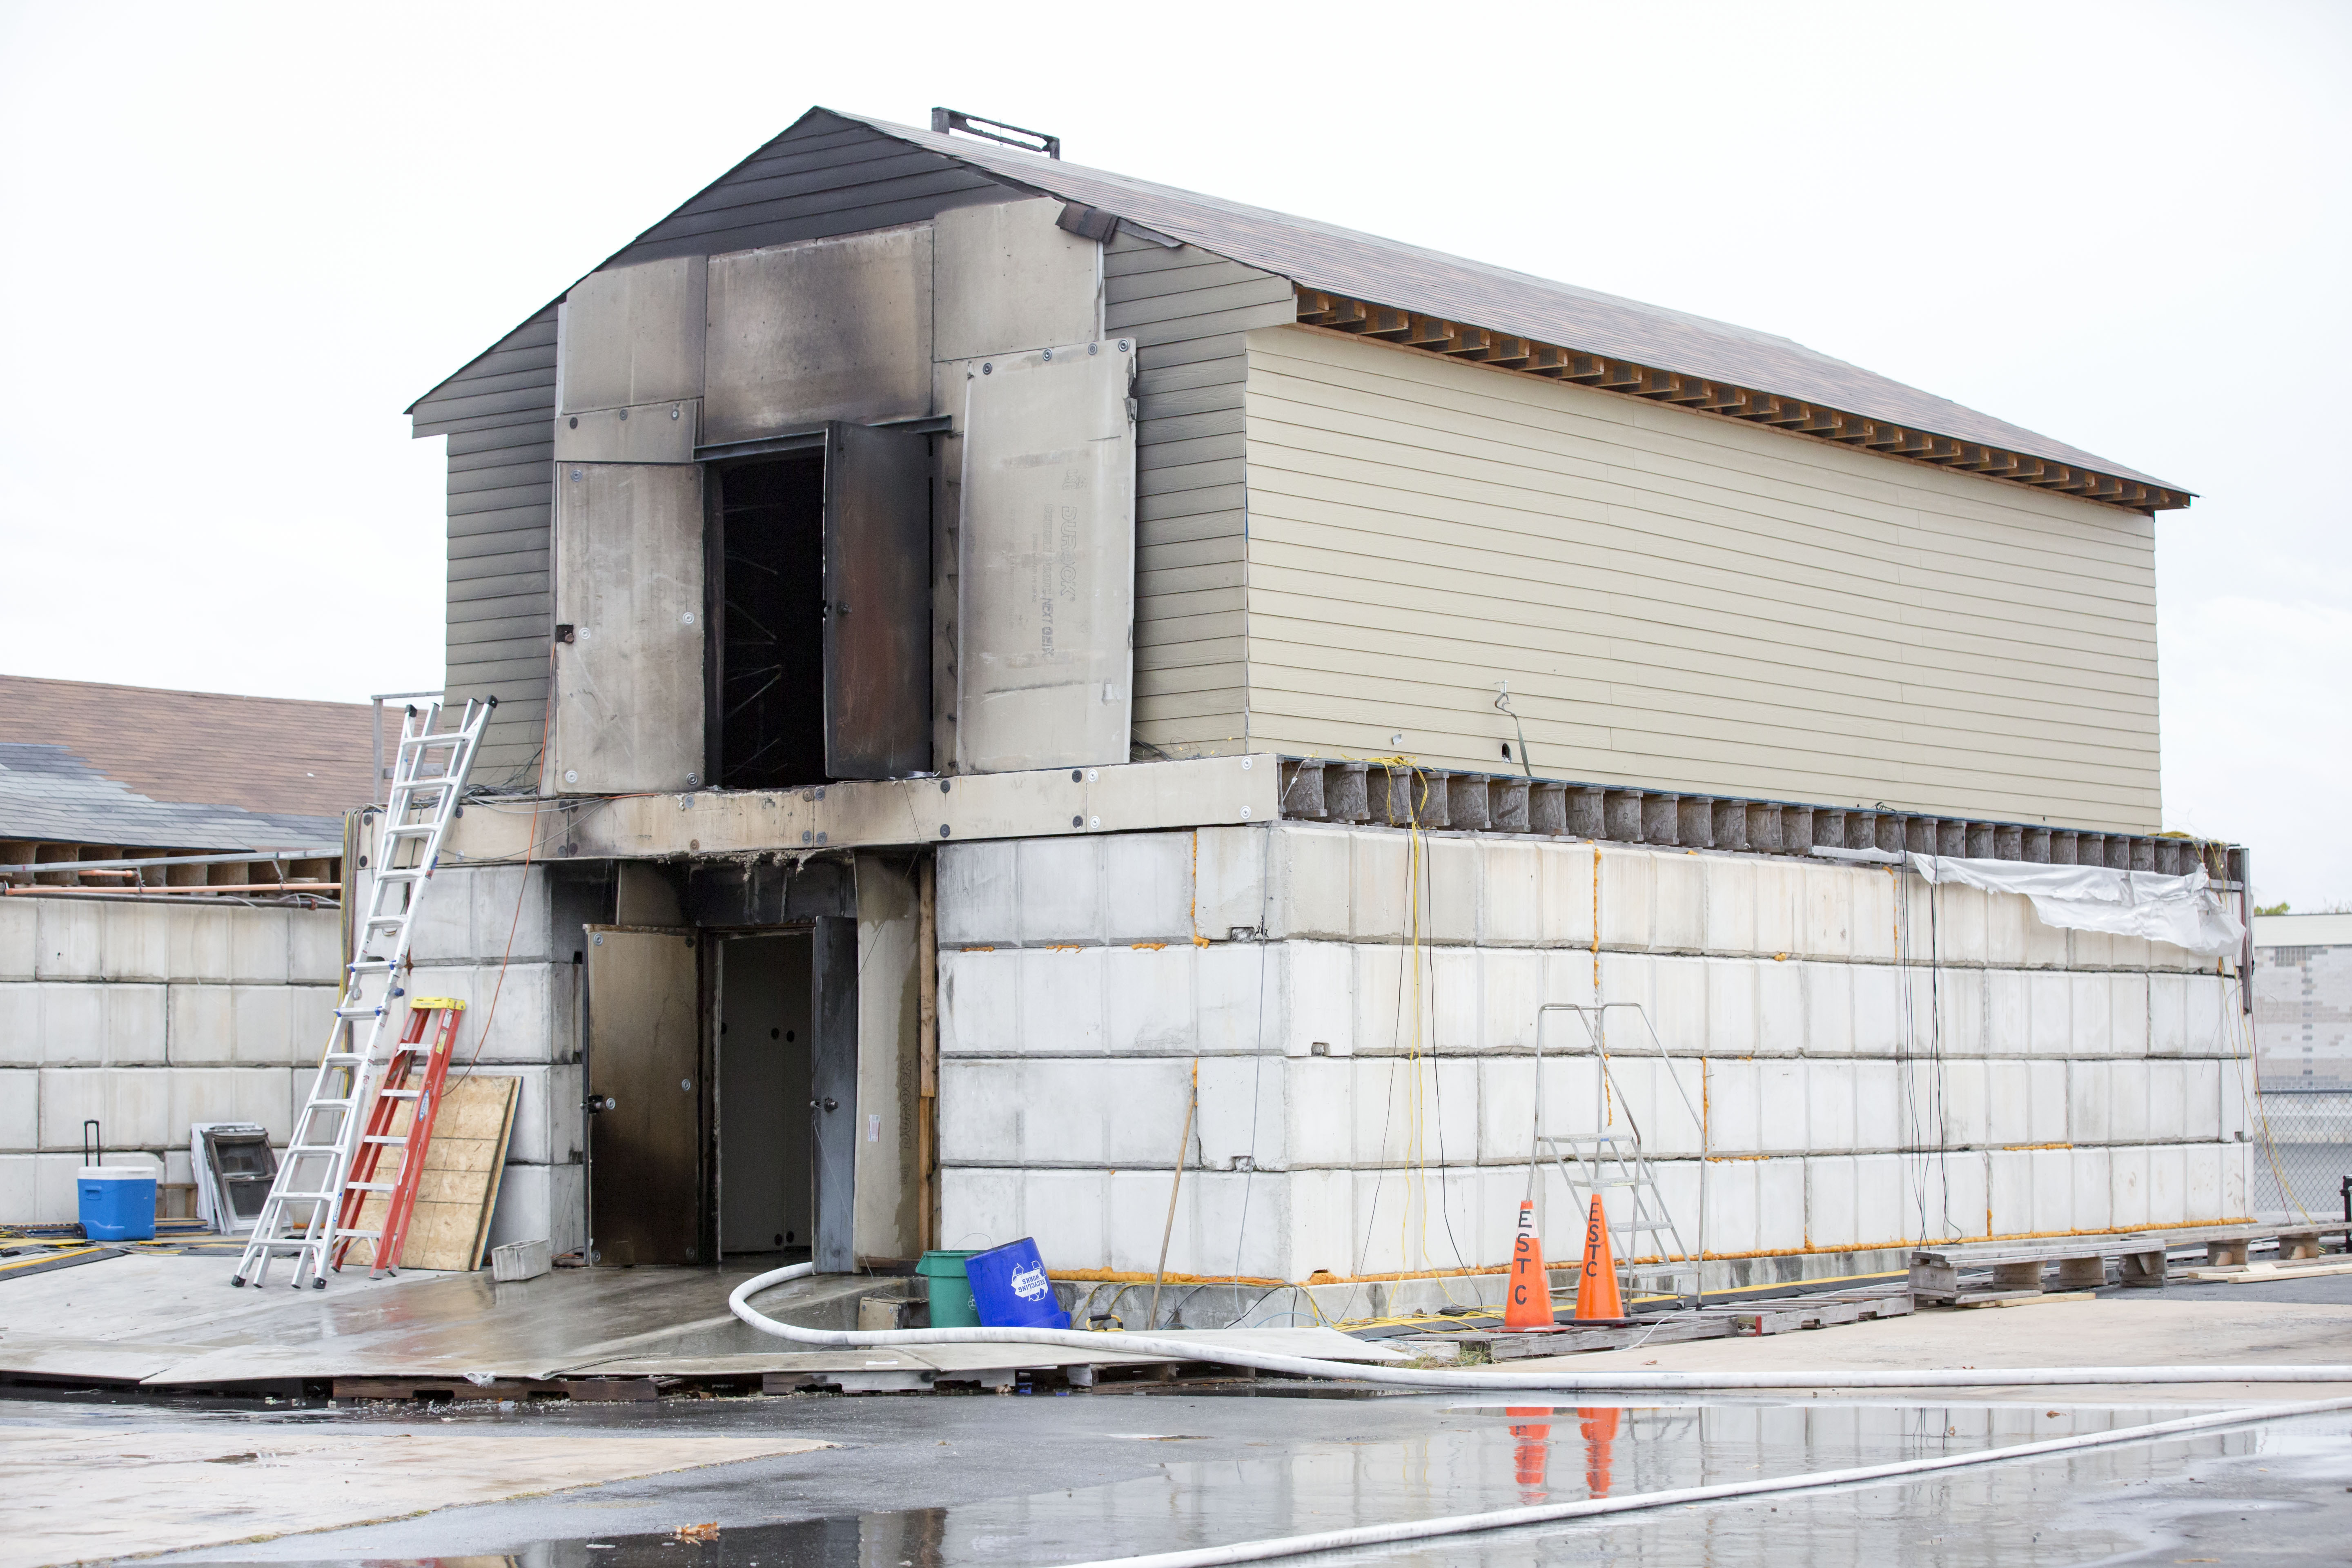
\includegraphics[width=\columnwidth]{Figures/Air_Entrainment/delcocorner.jpg}
	\caption{Delaware County, PA Fire Test Structure}
	\label{fig:Delaware_County,_PA_Fire_Test_Structure}
\end{figure}

The outer walls of the first floor of the structure were composed of interlocking concrete blocks 2~ft. wide, 2~ft. high, and 4~ft. long. The interior dimensions of the structure were 20~ft. wide, 36~ft. long, and 8~ft. high. The joints and gaps between the blocks were filled with high temperature insulation. The interior walls of the first floor were framed with steel studs set to 16~in. centers and track and were lined with 0.5~in. thick cement board. The walls were composed of 0.6~in. Type X gypsum board. Additionally, the ceiling was composed of two layers of 0.5~in. thick cement board. The first floor ceiling support of the structure was composed of wood truss joist I-beams (TJIs) with a 11.75~in. depth. Each TJI was composed of laminated veneer lumber flanges with a cross section of 1.13~in. x 1.75~in. and an 0.43~in. thick oriented strand board web. Tongue and groove oriented strand board of 0.72~in. thickness was screwed to the top of the TJIs. 

A stairwell was built to connect the two floors of the structure. The stairs had a 7.25~in rise and 7.5~in run and started 5.25~ft off the south wall with a width of 14~ft off the east wall. The second story walls were wood framed with 2~in by 4~in studs. The studs were set to 16~in centers. The interior walls were protected by 0.63~in fire rated gypsum board, 0.63~in Durock board, and a second layer of 0.63~in fire rated gypsum board. The exterior walls were protected with 0.31~in oriented strand board and 0.31~in fiber cement lap siding. Dimensioned drawings of the first and second floor are shown in Figures~\ref{fig:Delaware_County,_PA_Fire_Test_Structure_First_Floor} and \ref{fig:Delaware_County,_PA_Fire_Test_Structure_Second_Floor} respectively.

\begin{figure}[!ht]
	\centering
	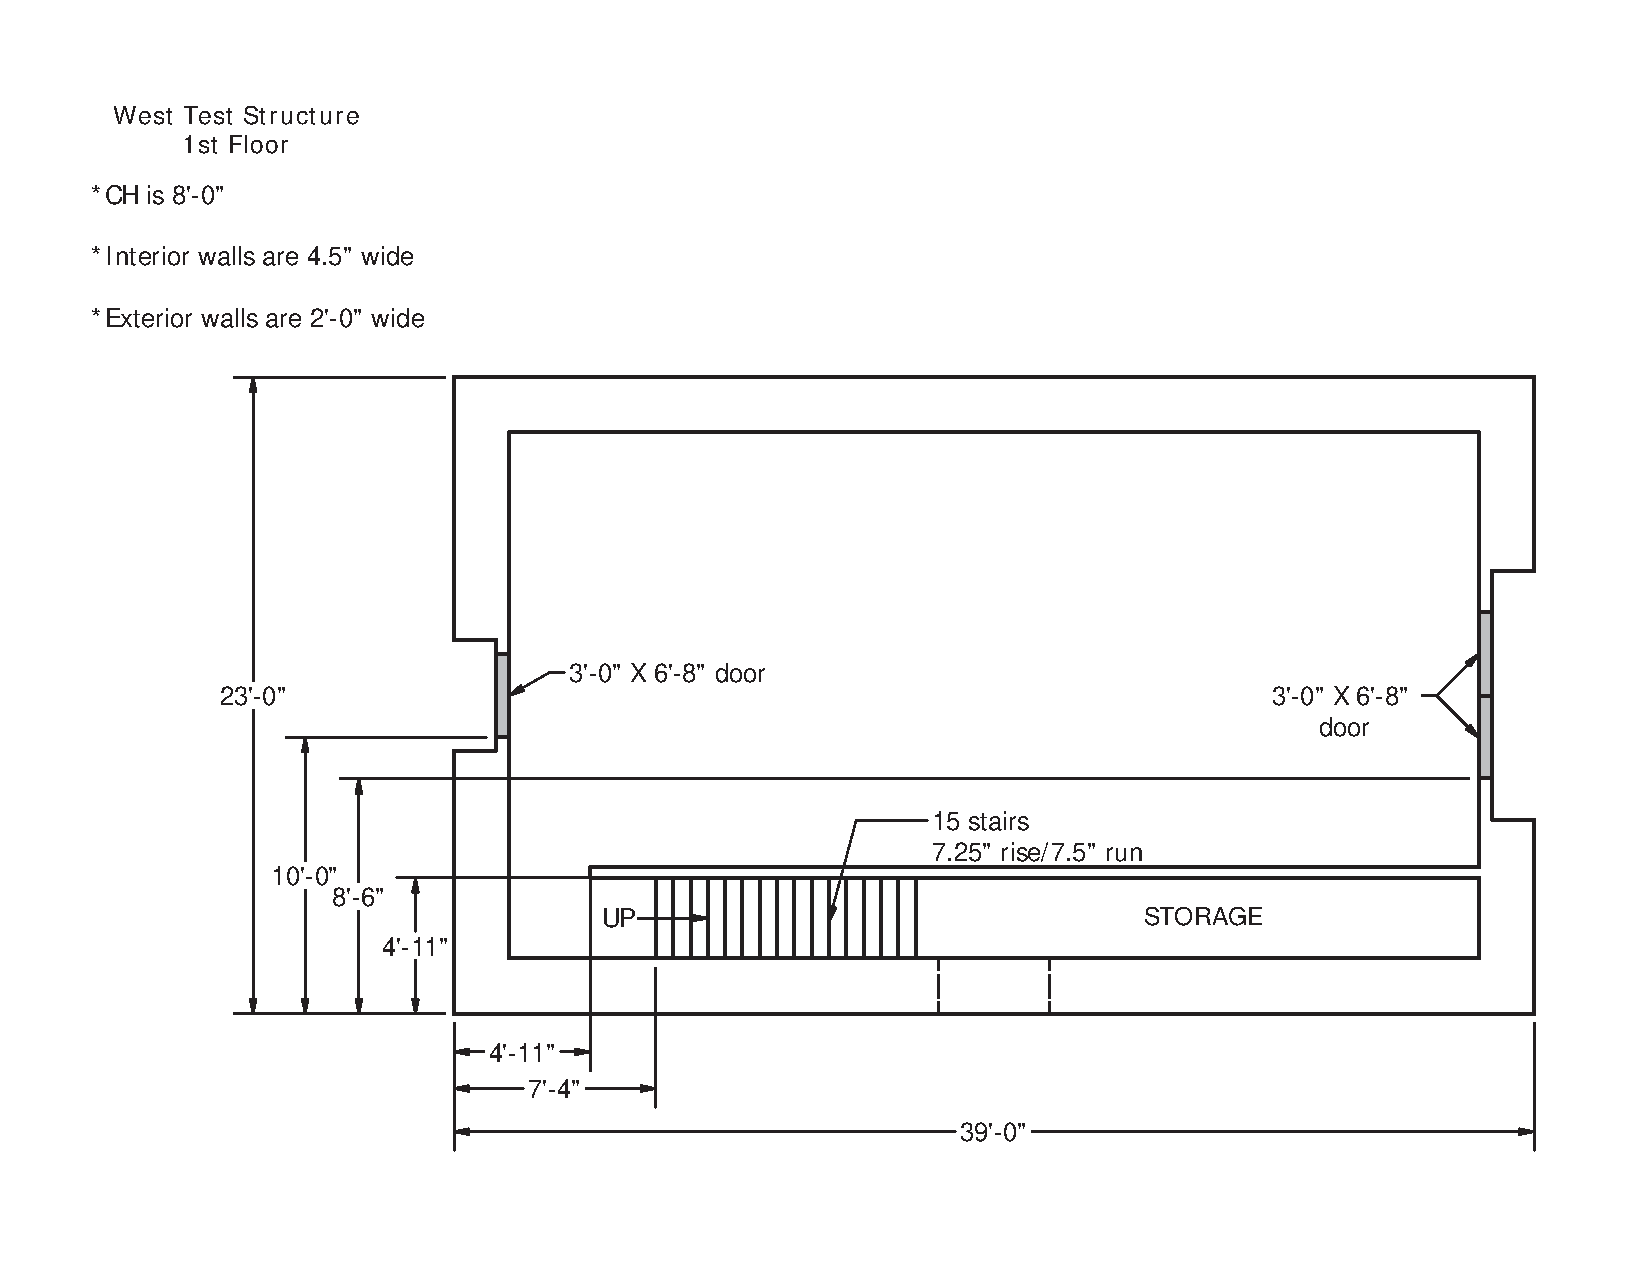
\includegraphics[width=\columnwidth]{Figures/Air_Entrainment/West_Test_Structure_1st_Floor_original_nodim.pdf}
	\caption{Delaware County, PA Fire Test Structure First Floor}
	\label{fig:Delaware_County,_PA_Fire_Test_Structure_First_Floor}
\end{figure}

\begin{figure}[!ht]
	\centering
	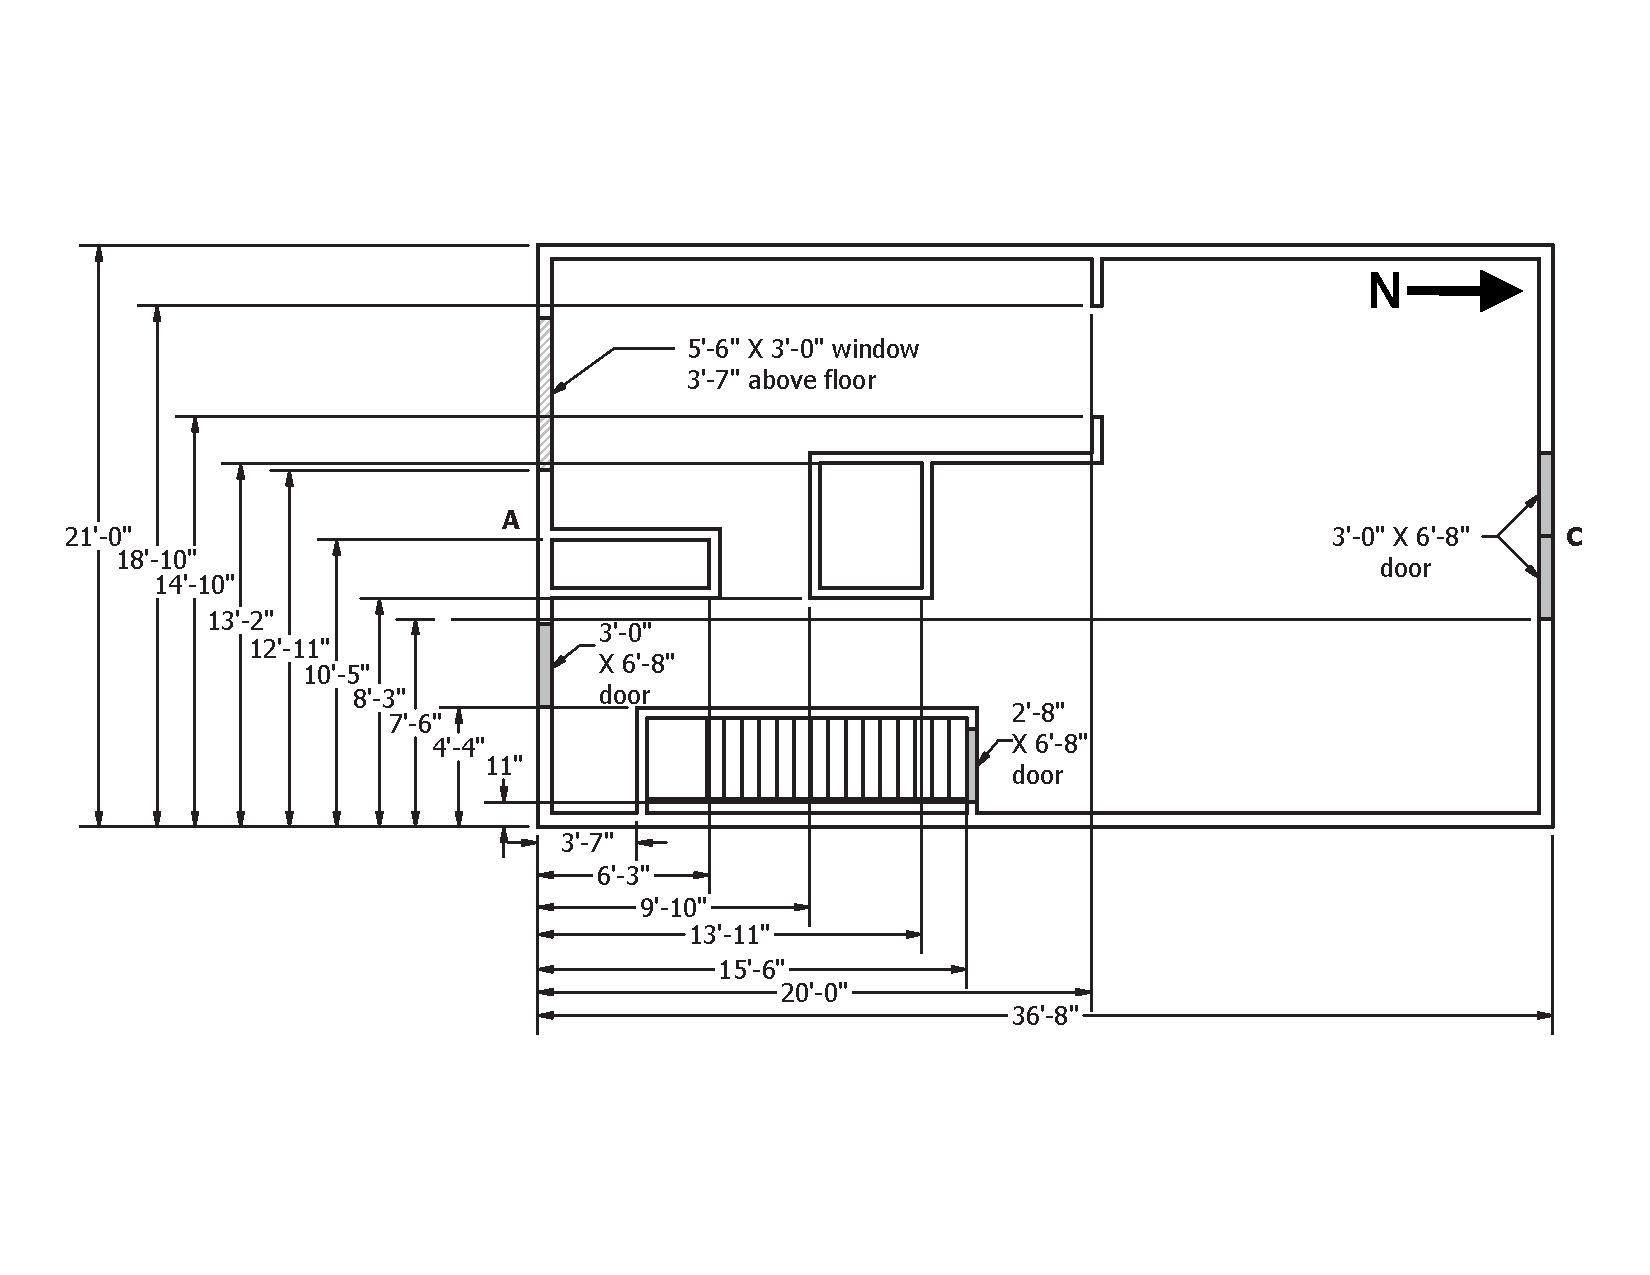
\includegraphics[width=\columnwidth]{Figures/Air_Entrainment/West_Test_Structure_2nd_Floor_nodim.pdf}
	\caption{Delaware County, PA Fire Test Structure Second Floor}
	\label{fig:Delaware_County,_PA_Fire_Test_Structure_Second_Floor}
\end{figure}

The exterior doorways of each structure were steel doors that were opened or closed at certain instances during tests to change the ventilation configuration within the structure. All other doorways in the structures did not contain a door. If it was determined that these doors needed closed during a test, a sheet of either gypsum board or oriented strand board was used to cover the opening and remained as such until the conclusion of the given test.

% A series of the air entrainment experiments involved a reconfiguration of the first floor of the structure. An interior dividing wall was constructed 10~ft-4~in. from the North wall the to compartmentalize th first floor. A standard 2~ft. 6~in. by 6~ft. 8~in. doorway was created 17~ft off the East wall to join the compartments. A 16~ft interior wall was added to the dividing wall to create a a hallway along the West side of the structure that was 16~ft by 4~ft. This allowed for the team to study entrainment in a structure configuration most comparable to residential single family homes. 

% \begin{figure}[!ht]
% 	\centering
% 	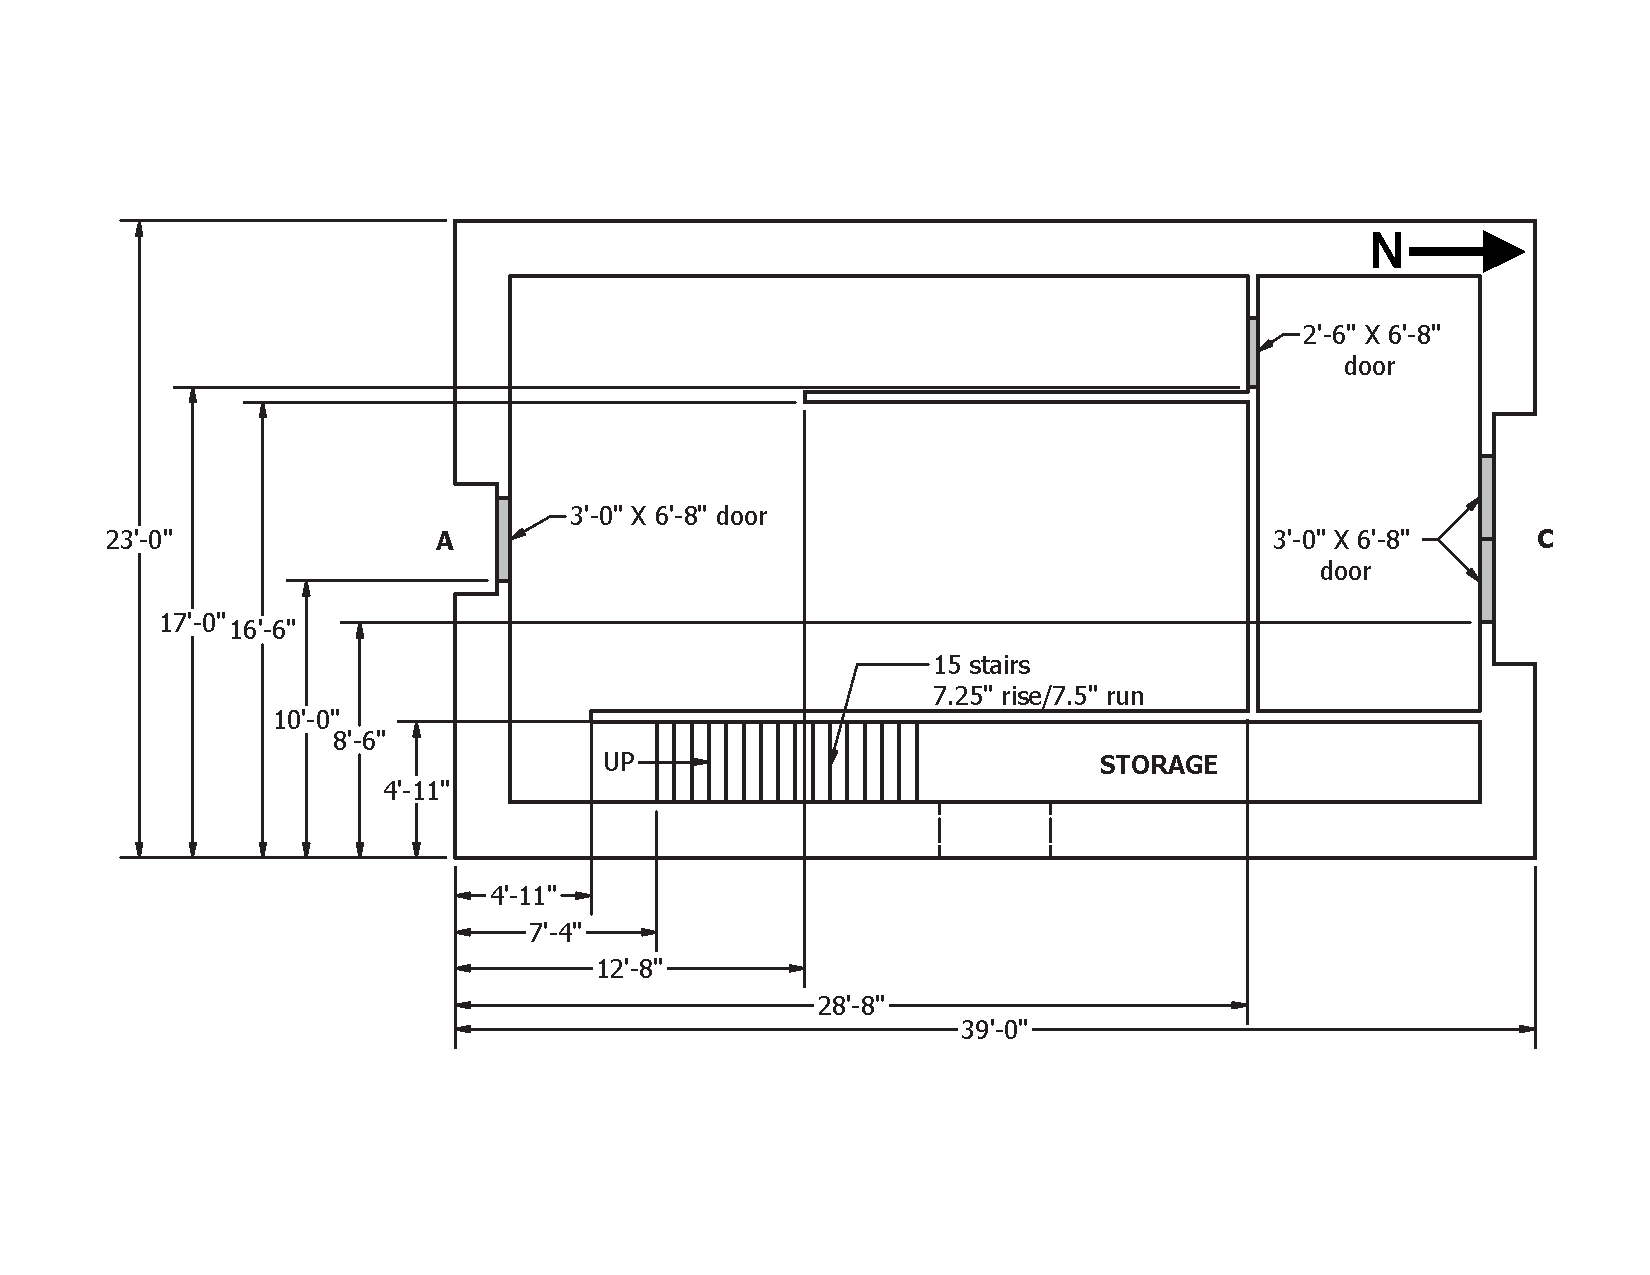
\includegraphics[width=\columnwidth]{Figures/Air_Entrainment/West_Test_Structure_1st_Floor_nodim.pdf}
% 	\caption{First Floor Alterations Room Configuration}
% 	\label{fig:First_Floor_Alterations_Room_Configuration}
% \end{figure}

\clearpage

\section{Equipment Used}

To ensure the data collected and associated results were applicable to the majority of the fire service, a list of representative nozzles, specified flow rates/pressures, and nozzle movement techniques was created. The variables, which were used during the air entrainment experiments are included in the Table~\ref{tab:Nozzle Selection}.

\begin{table}[!ht]
\centering
\caption{Nozzles Used In Testing}\label{tab:Nozzle Selection}
\begin{tabular}{llccc}
\toprule[1.5pt]
Line Size & Nozzle Type & Tip (in)& Nozzle Pressure (psi) & Approximate Flow Rate (gpm) \\
\midrule
1 3/4 in. & Smooth Bore & 1     & 50  & 210 \\
          & Smooth Bore & 15/16 & 50  & 180 \\
          & Smooth Bore & 7/8   & 50  & 150 \\
          & Combination &       & 50  & 150 \\
          & Combination &       & 75  & 150 \\
          & Combination &       & 100 & 100 \\
          & Combination &       & 100 & 150 \\
\midrule
2 1/2 in. & Smooth Bore & 1 1/8 & 50  & 260 \\
          & Smooth Bore & 1 1/4 & 50  & 320 \\
          & Combination &       & 50  & 250 \\ 
          & Combination &       & 75  & 250 \\
          & Combination &       & 100 & 250 \\
\bottomrule[1.25pt]
\end{tabular}
\end{table}

These experiments involved the repetition of nozzle movements and patterns; therefore to minimize nozzle operator fatigue and improve repeatability a nozzle prop was constructed. The prop was used as the `backup' firefighter by supporting the hoseline and minimizing nozzle reaction forces on the operator. Figure~\ref{fig:Nozzle_Prop} shows a dimensioned drawing and the constructed prop. The horizontal base and vertical member were constructed of 4'' by 4'' dimensioned lumber while the angled supports were constructed of 2'' by 6'' dimensioned lumber.

\begin{figure}[!ht]
\centering
    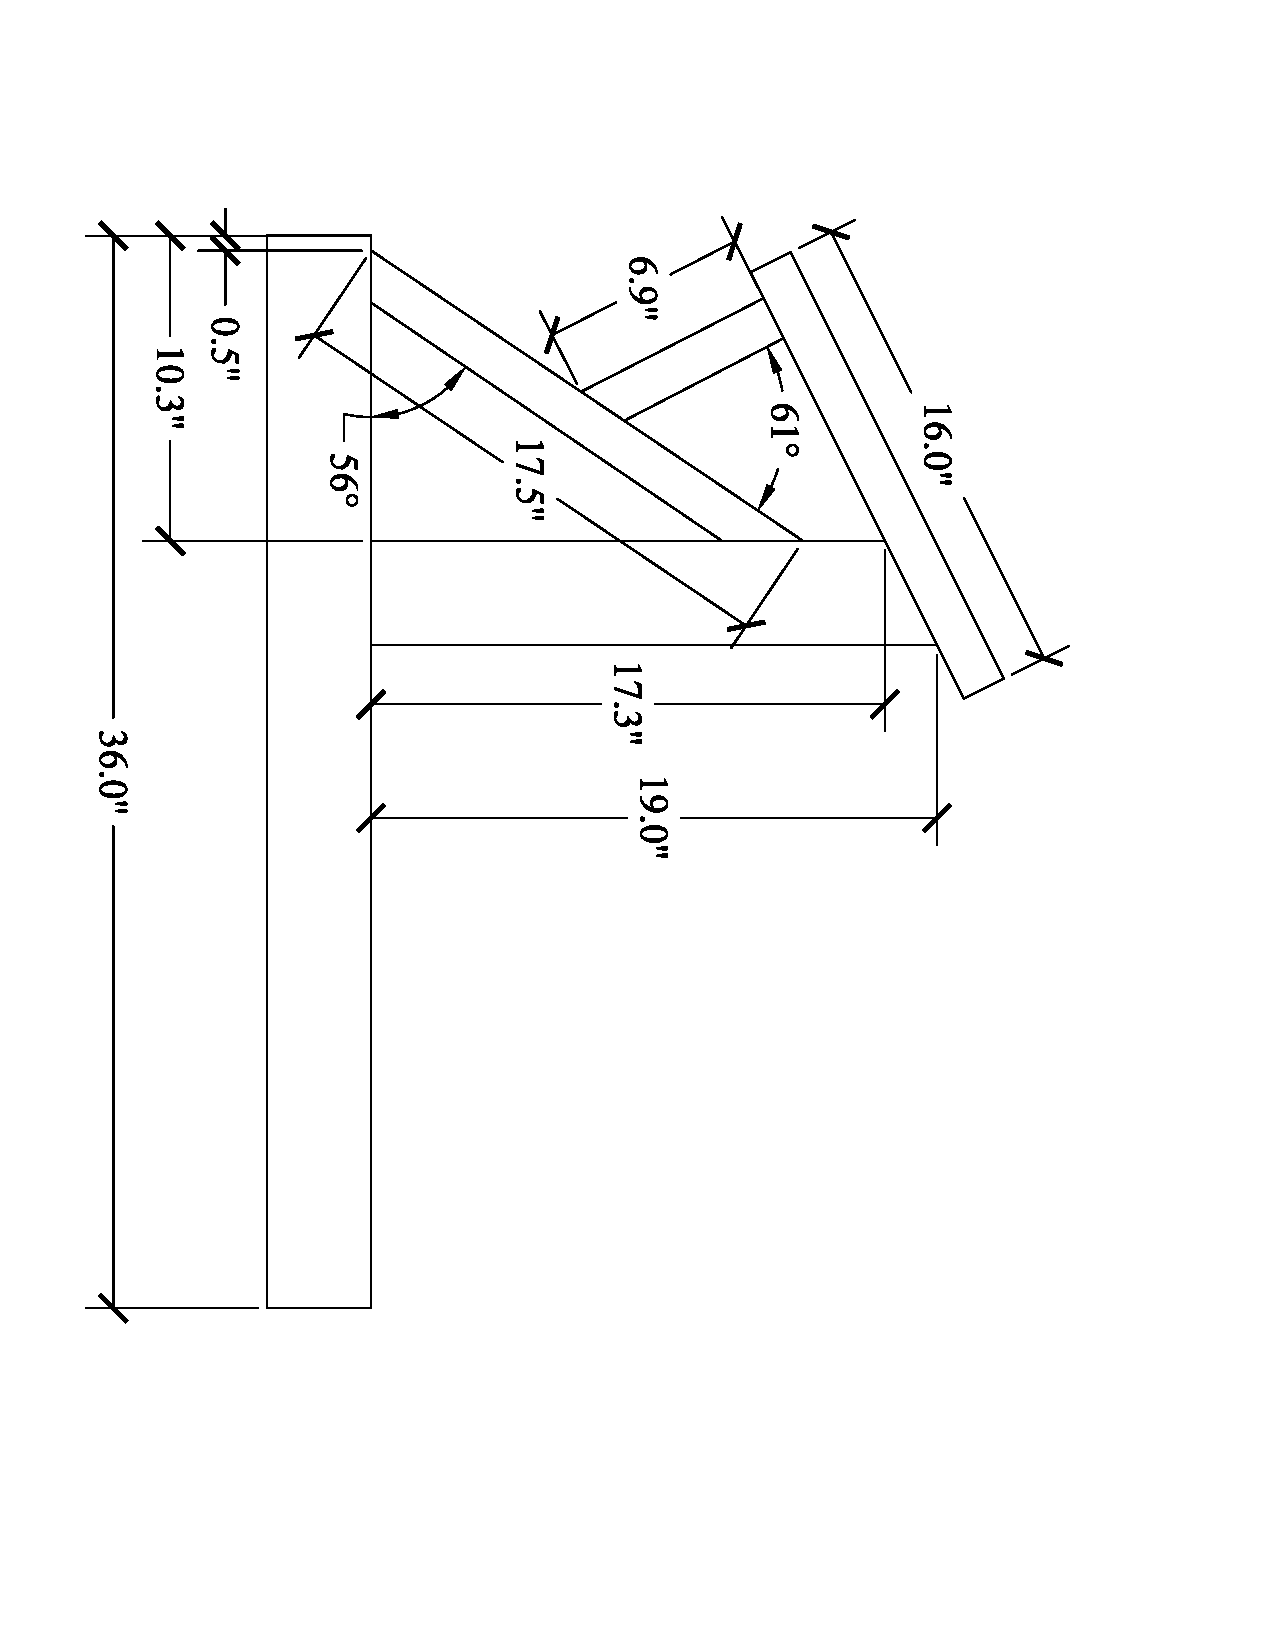
\includegraphics[width=.45\columnwidth]{Figures/Water_Distribution/GIBside}
	\includegraphics[width=.45\columnwidth]{Figures/Air_Entrainment/hoserig}
	\caption[Nozzle Prop]{Dimensioned drawing of the nozzle prop (left) and constructed prop (right).}
	\label{fig:Nozzle_Prop}
\end{figure}

The hose was affixed to the prop with `U' bolts and locking nuts to ensure the hose did not move during an experiment. The prop supported both 1.5~in. and 2.5~in. hoselines. To ensure the experiments were consistent (independent of variance of nozzle position on the prop), the distance from the nozzle to the ventilation opening was measured from the tip of the nozzle, and not the base of the prop.

\begin{figure}[!ht]
\centering
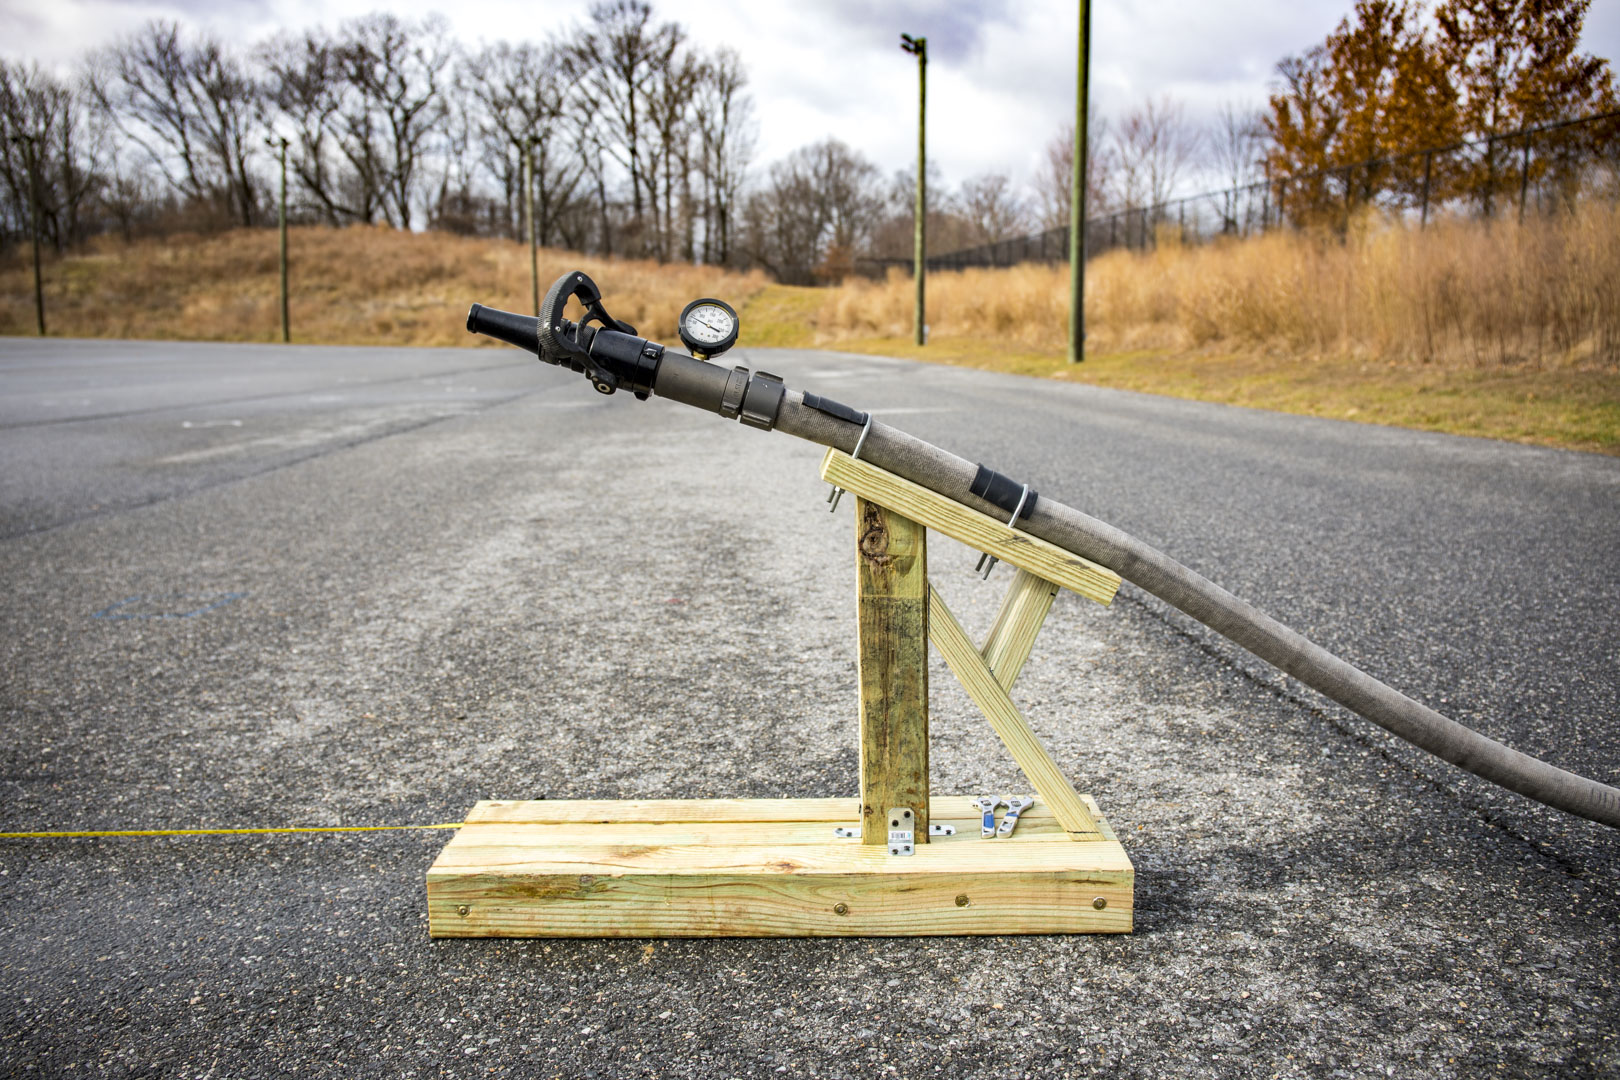
\includegraphics[width=.6\columnwidth]{Figures/Air_Entrainment/gib_hose} 
\caption{Nozzle Prop in Use}
\label{fig:Nozzle_Prop_in_Use}
\end{figure}

\section{Instrumentation and Uncertainty}
\label{sec:uncert}
Gas velocity, a measure of air entrainment by hose streams, was obtained through the use of an array of bi-directional probes. Bi-directional probes were connected to a pressure transducers to evaluate the change in pressure associated with the gas flow. The differential pressure transducer was a Setra Model 264 with a range of +/- 0.5~in. WC (+/- 124.5~Pa.). The uncertainty given by the manufacturer is 1\% or 1.2~Pa. 

A gas velocity measurement study examining the doorway flow of pre-flashover compartment fires yielded expanded uncertainty measurements ranging from $\pm$~0.14 to $\pm$~0.22 for bi-directional probes of similar design~\cite{Bryant:FSJ2009}. The total expanded uncertainty for gas velocity in these experiments is estimated to be $\pm$~18~\%.

\section{Measurement Location}
\label{sec:location}
There were several challenges associated with measuring air entrainment from hose streams. The first challenge existed because the experiments were conducted outside, therefore considering wind was critical. Additionally, the instrumentation used in data collection is best in a dry environment to maintain the smallest level of uncertainty and remain operational. To address these challenges, the measurement location was set at the doorway at the top of the stairwell. Figure~\ref{fig:Measurement_Location_Second_Floor} shows the position of the the bi-direction probe array on the second floor.

\begin{figure}[!ht]
	\centering
	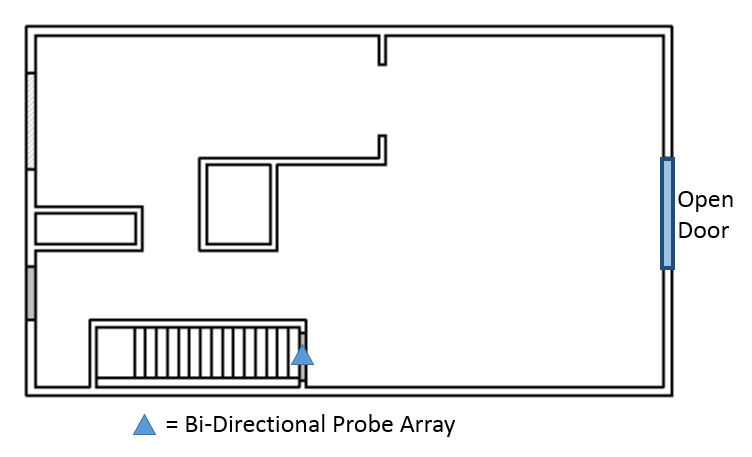
\includegraphics[width=.7\columnwidth]{Figures/Air_Entrainment/Measurement_Locations_Secondfloor}
	\caption{Measurement Location (Second Floor)}
	\label{fig:Measurement_Location_Second_Floor}
\end{figure}

Figures~\ref{fig:Air_Entrainment_Flowpath_Interior_Experiments} and \ref{fig:Air_Entrainment_Flowpath_Exterior_Experiments} show the experimental configuration for the interior flow tests and exterior flow tests, respectively. The arrows indicate the flow direction based on the hose stream being the source of the flow through air entrainment.

\begin{figure}[!ht]
	\centering
	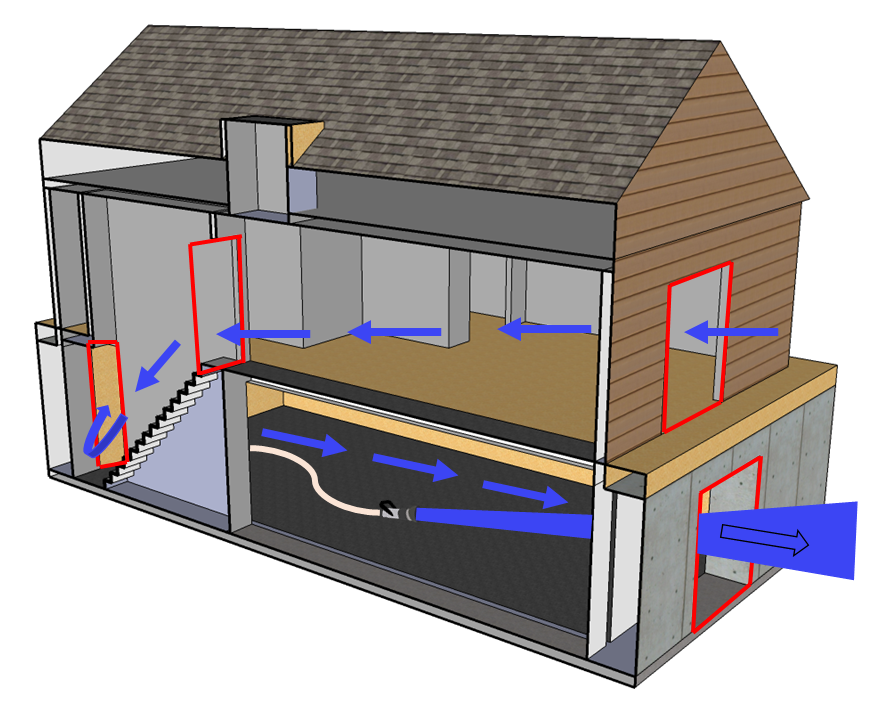
\includegraphics[width=.7\columnwidth]{Figures/Air_Entrainment/Airflow_Layout}
	\caption{Air Entrainment Flowpath, Interior Experiments}
	\label{fig:Air_Entrainment_Flowpath_Interior_Experiments}
\end{figure}

\begin{figure}[!ht]
	\centering
	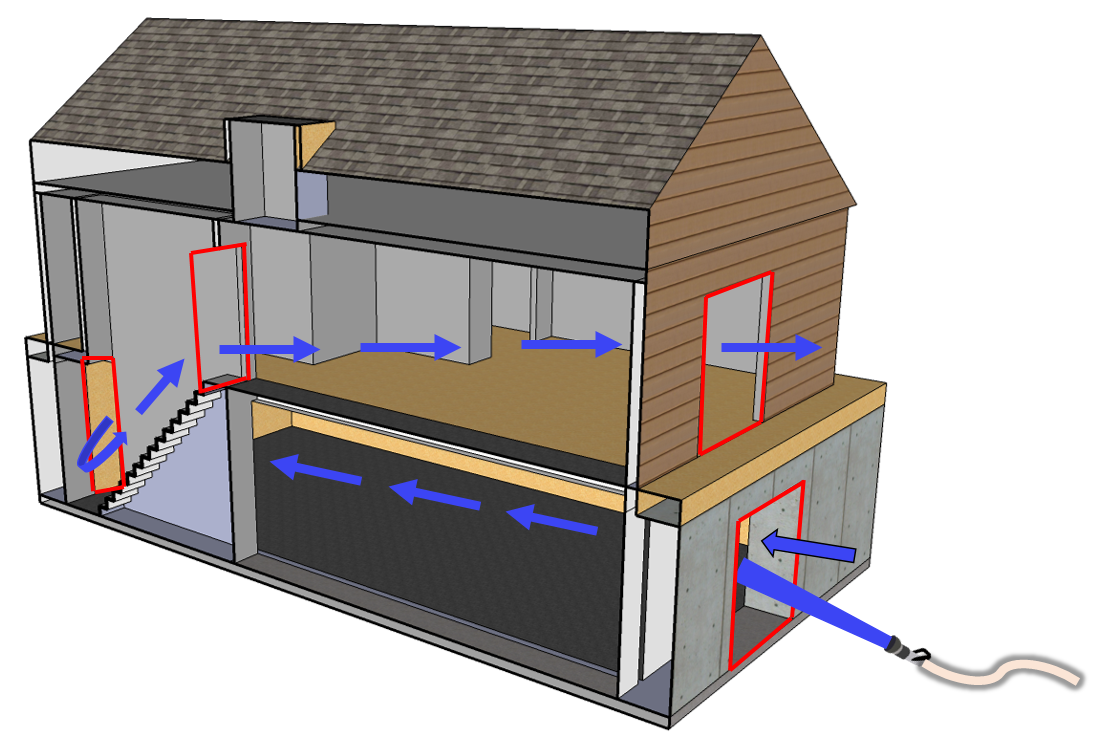
\includegraphics[width=.7\columnwidth]{Figures/Air_Entrainment/Airflow_Layout_Ext}
	\caption{Air Entrainment Flowpath, Exterior Experiments}
	\label{fig:Air_Entrainment_Flowpath_Exterior_Experiments}
\end{figure}

The measurement location was placed at the top of the stairs, within the flow path of both test configurations. This location kept the instrumentation dry and out of the reach of a hose stream. While this location did not guarantee isolation from wind effects due to open vents, this represented the best location to minimize those effects.

\clearpage

\section{Flow Locations}

For the base configuration of the experimental facility (Figures~\ref{fig:Delaware_County,_PA_Fire_Test_Structure_First_Floor} and \ref{fig:Delaware_County,_PA_Fire_Test_Structure_Second_Floor}), there were two main locations where the hoses were placed to flow water: interior and exterior. For an interior test, the nozzle was set to be 12~ft from the doorway on the first floor of the structure and water flowed from that position through the open vent, out of the structure (Figure~\ref{fig:First_Floor_Setup_Total_Entrainment_Interior_Tests}). For the exterior tests, the nozzle was again set 12~ft from the first floor doorway but water flowed from the exterior of structure through the vent into the first floor of the structure (Figure~\ref{fig:First_Floor_Setup_Total_Entrainment_Exterior_Tests}). This had the global effect of either pulling air passed the measurement array on the second floor or pushing air passed the the measurement array for the interior and exterior locations respectively.

\begin{figure}[!ht]
	\centering
	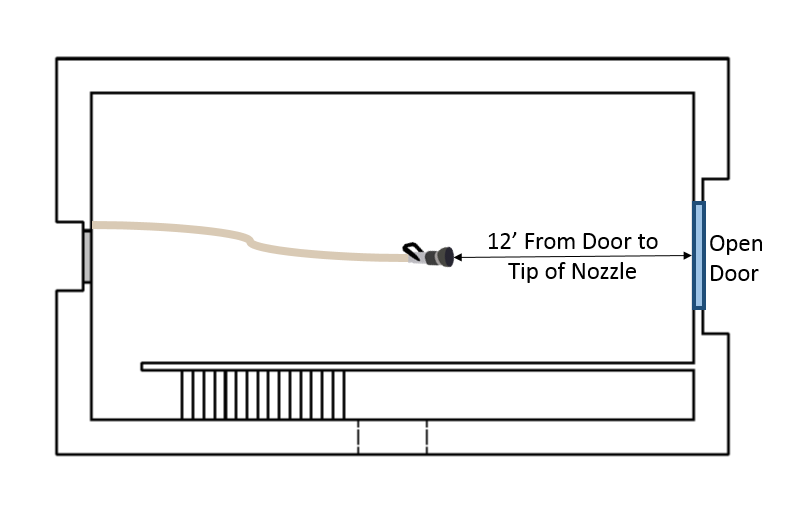
\includegraphics[width=.6\columnwidth]{Figures/Air_Entrainment/Measurement_Locations_Firstfloor}
	\caption{First Floor Setup - Total Entrainment Interior Tests}
	\label{fig:First_Floor_Setup_Total_Entrainment_Interior_Tests}
\end{figure}

\begin{figure}[!ht]
	\centering
	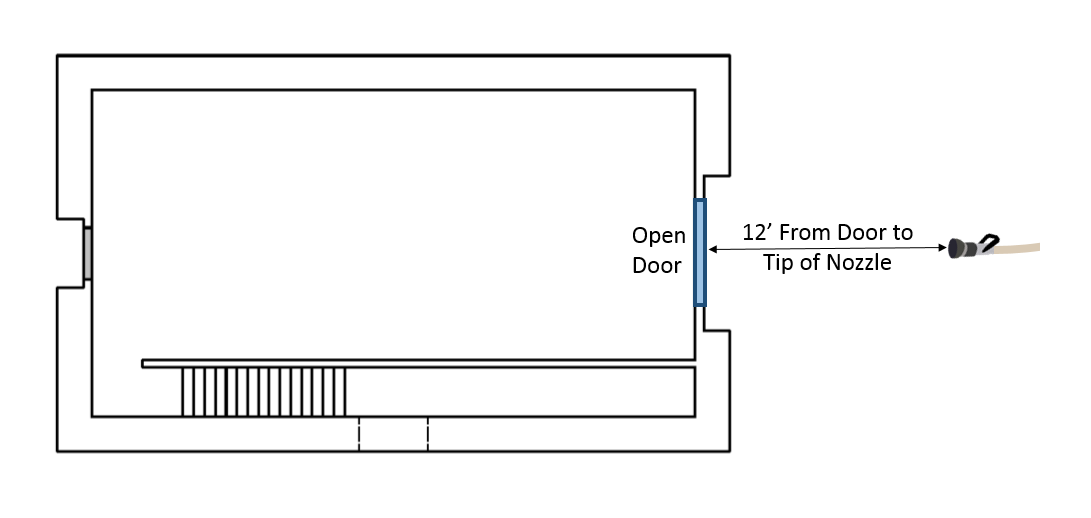
\includegraphics[width=.95\columnwidth]{Figures/Air_Entrainment/Measurement_Locations_Firstfloor_Ext}
	\caption{First Floor Setup - Total Entrainment Exterior Tests}
	\label{fig:First_Floor_Setup_Total_Entrainment_Exterior_Tests}
\end{figure}

% The air entrainment experiments that involved the reconfiguration the first floor of the structure (Figure~\ref{fig:First_Floor_Alterations_Room_Configuration}) were also interior tests (water was flown from the inside of the structure to the outside). These experiments featured both a fixed position nozzle and advancing nozzle position (moving toward the exit along the interior hallway). Figure~\ref{fig:First_Floor_Setup_Total_Entrainment_Exterior_Tests} shows the fixed position of the nozzle and the open vents. For advancing experiments, the nozzle moved toward the open door.

% \begin{figure}[!ht]
% 	\centering
% 	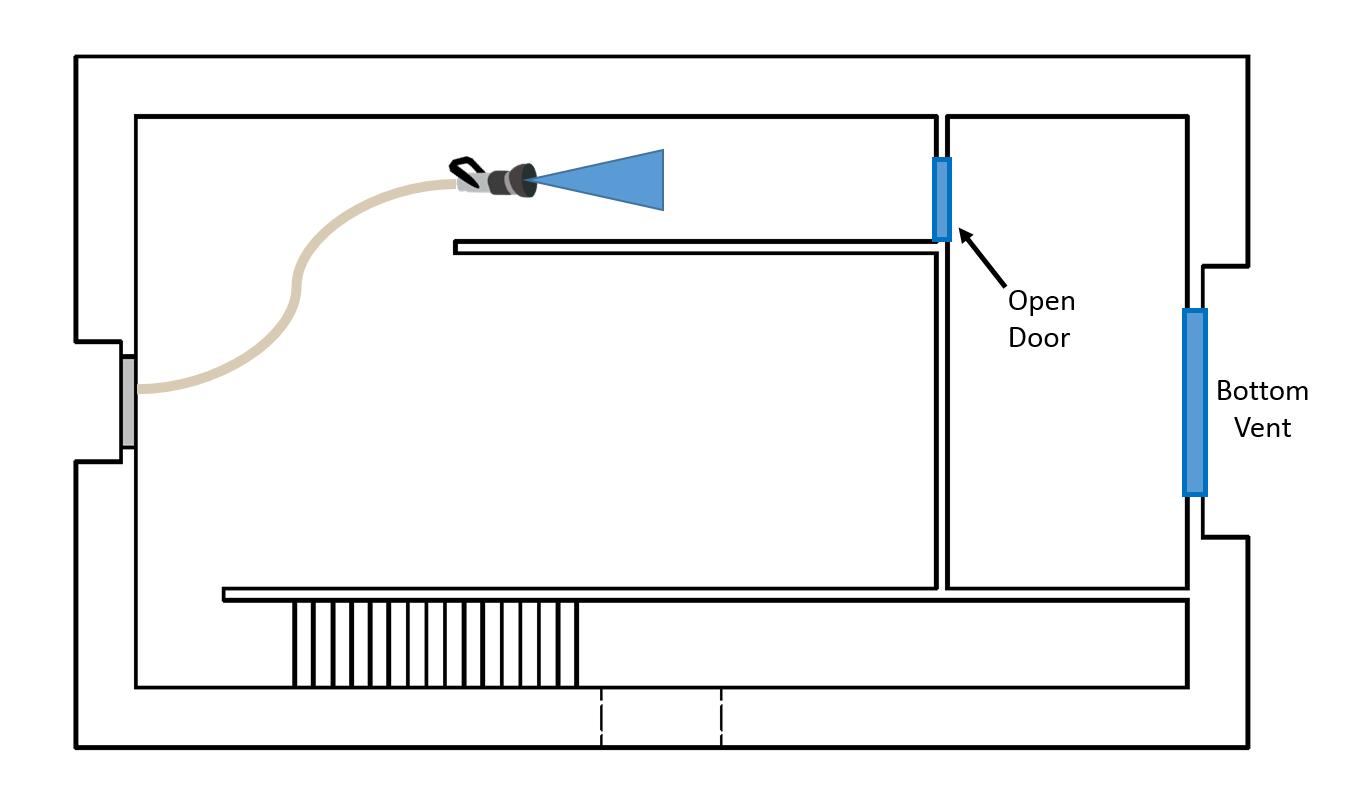
\includegraphics[width=.6\columnwidth]{Figures/Air_Entrainment/Measurement_Location_Room_Configuration_Bottom}
% 	\caption{First Floor Room Configuration, Interior Experiments}
% 	\label{fig:First_Floor_Room_Configuration_Interior_Experiments}
% \end{figure}


\chapter{Experiments Conducted}

Experiments were completed to determine how air entrainment from hose streams was affected by varying equipment, spray patterns, hose stream type, and ventilation. In each experimental configuration, water flowed for approximately 60~s. An average velocity was calculated at the measurement location (Section~\ref{sec:location}) using the bi-directional probes and the average velocity multiplied by the measurement area to calculate a volumetric flow rate in cubic feet per minute (CFM). To compare different configurations, an average flow rate was calculated over the duration for each specific configuration. Figure~\ref{fig:cfmplotexplainer} shows the entrained air in volumetric flow as a function of time (dashed line) and the time-averaged flow rate between `events' (solid line). The time-averaged value was calculated between each event call-out and the value is tied to the event call-out on the left side of the interval. During each test, approximately 60~s of background data was taken so the ambient conditions could be isolated from experimental data. After ambient fluctuations were accounted for, the average volumetric flow during the background event was approximately 0~CFM. When the straight stream flow was started in Figure~\ref{fig:cfmplotexplainer}, the average CFM during that event jumped to approximately 1700~CFM. Note that while the transient (dashed) data shows fluctuations typical of velocity data, the magnitudes of the fluctuations did not prevent distinct events from being distinguishable.

\begin{figure}[!ht]
\centering
\includegraphics[width=.8\columnwidth]{Script_Figures/Entrainment/Exp_07_102615_CFM} 
\caption[Time History of Entrainment Experiment]{Time history of an entrainment experiment. The dashed line is the spatially averaged flow while the solid line represents the time average in the interval bounded by the vertical time callout lines.}
\label{fig:cfmplotexplainer}
\end{figure}

Based on the discussion in Section~\ref{sec:uncert}, the uncertainty associated with measurements from the bi-directional probes is $\pm$~18~\%. Therefore, the time-averaged air entrainment data has uncertainty bars included (cf. Figure~\ref{fig:cfmbarexplainer}). For the data where the the uncertainty bars overlap, such as those in the Figure~\ref{fig:cfmbarexplainer}, the differences between the CFM averages cannot be differentiated. 

\begin{figure}[!ht]
\centering
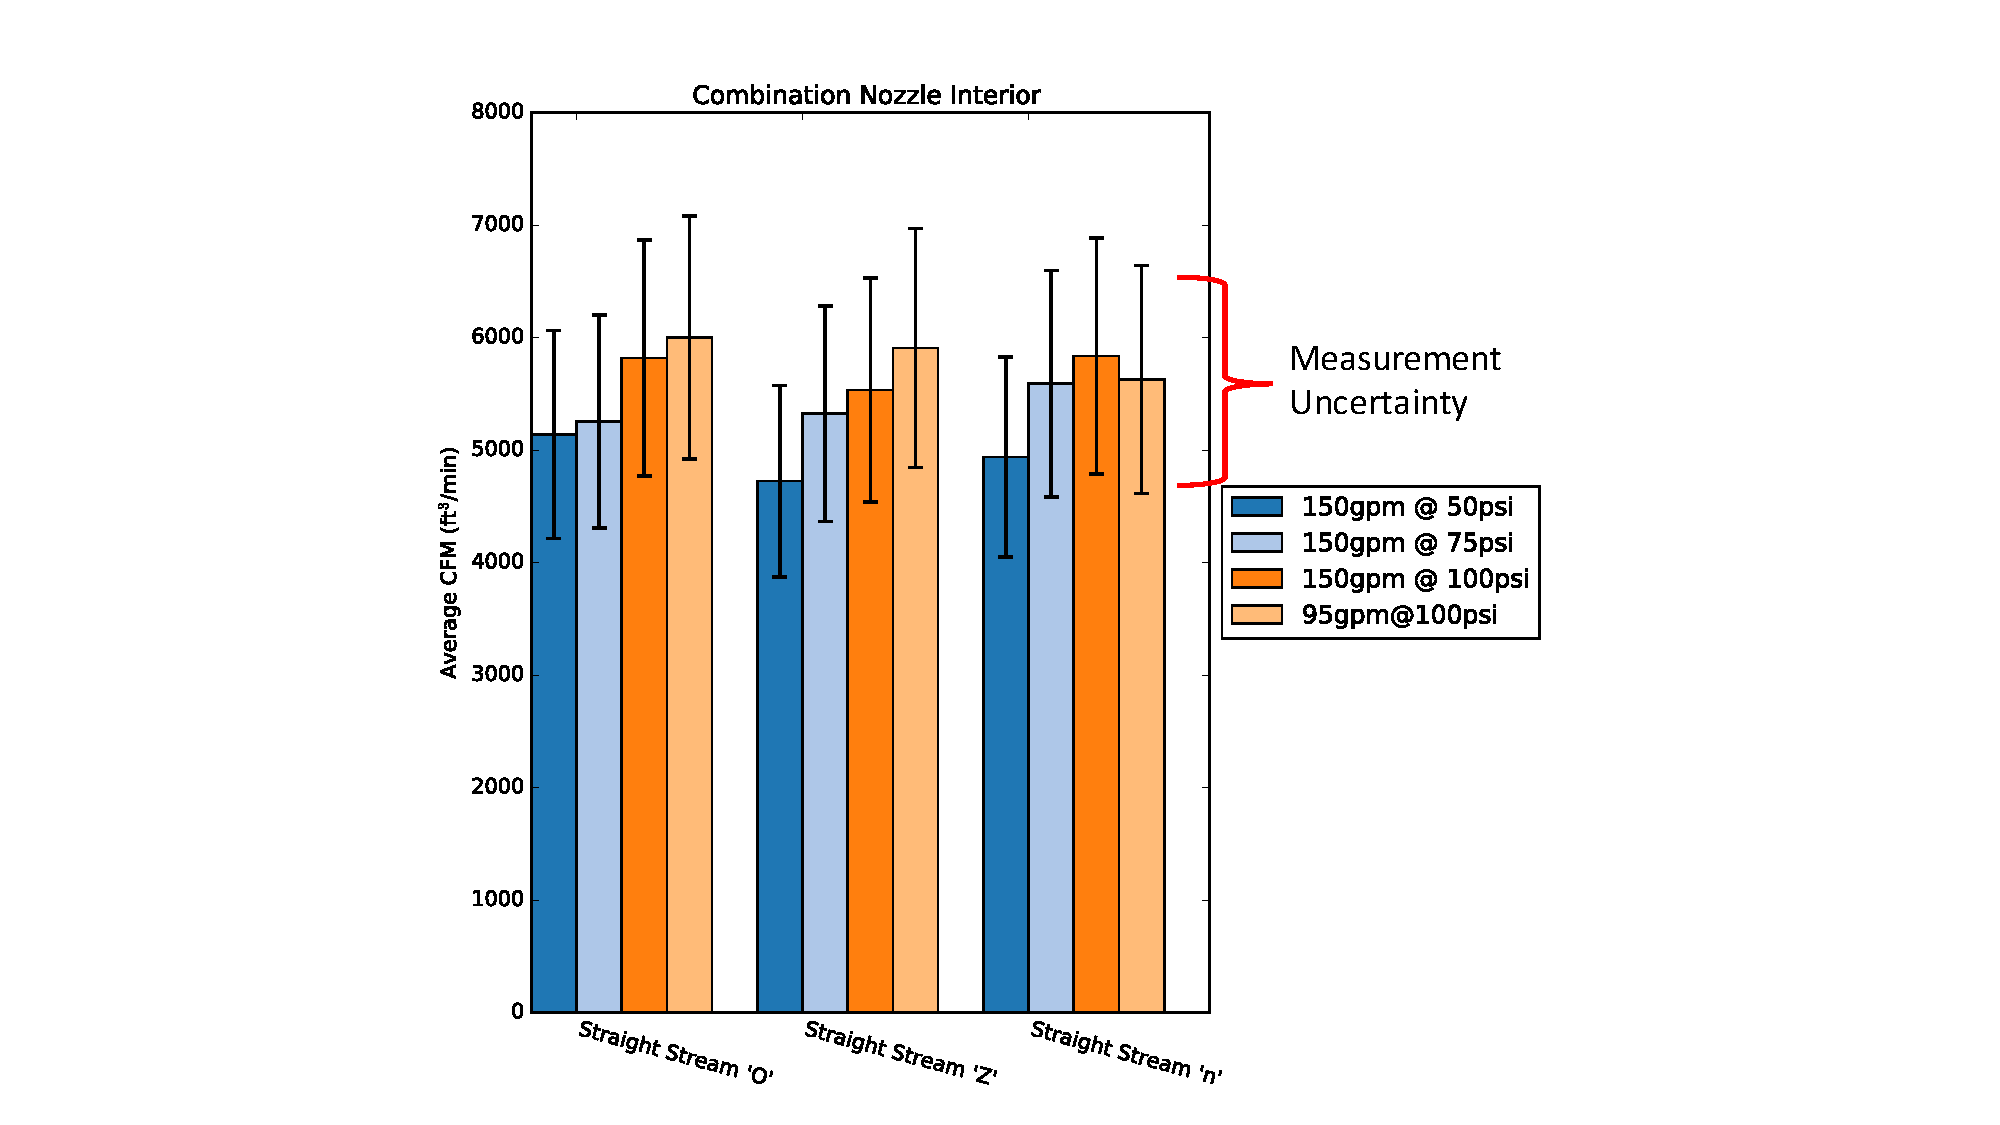
\includegraphics[width=.8\columnwidth]{Figures/Air_Entrainment/Total_Entrainment_Example} 
\caption[Average Flow Rate Comparison]{Example of bar chart comparisons with uncertainty.}
\label{fig:cfmbarexplainer}
\end{figure}

\clearpage

\section{Manufacturer Comparison}

Experiments varying pressure/flow rate, hose stream type, and nozzle movement were conducted to quantify potential differences in air entrainment associated with using three three different manufacturer's nozzles (MFI, MFII, and MFIII). Table~\ref{tab:Manufacturer_Comparison_Experiments} shows the configurations examined. For all three hose stream types, both a fixed pattern and an `O' pattern were used from the interior position.

\begin{table}[!ht]
\centering
\caption{Manufacturer Comparison Experiments}
\label{tab:Manufacturer_Comparison_Experiments}
\begin{tabular}{cccc}
\toprule[1.5pt]
Hose Stream Type & Tip Size & Flow Rate & Pressure \\ 
\midrule
Straight Stream &       & 150 & 50 \\
Straight Stream &       & 150 & 75 \\
Straight Stream &       & 150 & 100 \\
Narrow Fog      &       & 150 & 50 \\
Narrow Fog      &       & 150 & 75 \\
Narrow Fog      &       & 150 & 100 \\
Smooth Bore     & 7/8   & 150 & 50 \\
Smooth Bore     & 15/16 & 180 & 50 \\
Smooth Bore     & 1     & 210 & 50 \\
\bottomrule[1.25pt]
\end{tabular}
\end{table}

Figure~\ref{fig:1_5_Interior_Combination_Manufacturer} shows the average flow rate (CFM) for both the straight stream and narrow fog hose stream types with fixed and `O' patterns under three different pressures: 50~psi, 75~psi, and 100~psi. Figure~\ref{fig:1_5_Interior_Smooth_Bore_Manufacturer} shows the average flow rate for three smooth bore nozzles; a 7/8~in. tip with 150~gpm at 50~psi, a 15/16~in. tip with 180~gpm at 50~psi, and a 1~in. tip with 210~gpm at 50~psi for both a fixed and `O' pattern.

\begin{figure}[!ht]
\begin{tabular*}{\textwidth}{lr}
\includegraphics[width=.5\columnwidth]{Script_Figures/Entrainment/Manufacturer_1_5_Combination_Nozzle_150gpm_50psi} &
\includegraphics[width=.5\columnwidth]{Script_Figures/Entrainment/Manufacturer_1_5_Combination_Nozzle_150gpm_75psi} \\
\end{tabular*}
\centering
\includegraphics[width=.5\columnwidth]{Script_Figures/Entrainment/Manufacturer_1_5_Combination_Nozzle_150gpm_100psi}
\caption[Average Air Entrainment Varying Manufacturer with Combination Nozzles]{Comparison of air entrainment results of three manufacturers for straight stream and narrow fog stream in fixed and `O' patterns with 150~gpm and 50~psi (upper left), 75~psi (upper right), and 100~psi (bottom).}
\label{fig:1_5_Interior_Combination_Manufacturer}
\end{figure}

\begin{figure}[!ht]
\begin{tabular*}{\textwidth}{lr}
\includegraphics[width=.5\columnwidth]{Script_Figures/Entrainment/Manufacturer_1_5_Smooth_Bore_Nozzle_7_8_150gpm_50psi} &
\includegraphics[width=.5\columnwidth]{Script_Figures/Entrainment/Manufacturer_1_5_Smooth_Bore_Nozzle_15_16_180gpm_50psi} \\
\end{tabular*}
\centering
\includegraphics[width=.5\columnwidth]{Script_Figures/Entrainment/Manufacturer_1_5_Smooth_Bore_Nozzle_1_210gpm_50psi} 
\caption[Average Air Entrainment Varying Manufacturer with Smooth Bore Nozzles]{Comparison of air entrainment results of three manufacturers for smooth bore stream in fixed and `O' patterns with 7/8~in. tip with 150~gpm at 50~psi (upper left), with 15/16~in. tip with 180~gpm at 50~psi (upper right), and 1~in. tip with 210~gpm at 50~psi (bottom).}
\label{fig:1_5_Interior_Smooth_Bore_Manufacturer}
\end{figure}

For the straight streams and narrow fog streams with both fixed patterns and `O' patterns, Figure~\ref{fig:1_5_Interior_Combination_Manufacturer}, the air entrainment for the three manufacturers was within the experimental uncertainty of the measurement for all three pressures. For the smooth bore streams, the three manufactures were generally within the experimental uncertainty of the air entrainment measurements (Figure~\ref{fig:1_5_Interior_Smooth_Bore_Manufacturer}). MFI had slightly lower average CFM for a fixed stream with 15/16~in. tip with 180~gpm at 50~psi and an `O' Pattern with a 1~in. tip with 210~gpm at 50~psi. While these two cases had lower average air entrainment, when assessing the magnitude of the differences over the set of comparisons made, the three manufacturers are similar. As a result, the experiments designed to assess the configuration variables all used nozzles from MFI. These experiments were grouped by using the baseline structure configuration and subsequently modified ventilation openings. %, and a modified first floor configuration.

\clearpage

\section{Baseline Structure Configuration}
The baseline structure configuration was to have open double doors on the first and second floor. With this structure configuration, the hose stream type, nozzle pattern, flow location, flow rate and pressure, and line size diameter were varied. Table~\ref{tab:Total_Air_Entrainment_Experiments} shows a list parameters studied within this structure configuration.

\begin{table}[!ht]
\centering
\caption{Air Entrainment Experiments}
\label{tab:Total_Air_Entrainment_Experiments}
\begin{tabular}{lcccccc}
\toprule[1.5pt]
Location & Line Size (in) & Nozzle Type & Tip Size & Flow Rate & Pressure \\ 
\midrule
Interior & 1~3/4 & Combination &       & 95 & 100 \\
Interior & 1~3/4 & Combination &       & 150 & 50 \\
Interior & 1~3/4 & Combination &       & 150 & 75 \\
Interior & 1~3/4 & Combination &       & 150 & 100 \\
Interior & 1~3/4 & Smooth Bore & 7/8   & 150 & 50 \\
Interior & 1~3/4 & Smooth Bore & 15/16 & 180 & 50 \\
Interior & 1~3/4 & Smooth Bore & 1     & 210 & 50 \\
\midrule
Interior & 2~1/2 & Combination &       & 250 & 50 \\
Interior & 2~1/2 & Combination &       & 250 & 75 \\
Interior & 2~1/2 & Combination &       & 250 & 100 \\
Interior & 2~1/2 & Smooth Bore & 1 1/8 & 260 & 50 \\
Interior & 2~1/2 & Smooth Bore & 1 1/4 & 320 & 50 \\
\midrule
Exterior & 1~3/4 & Combination &       & 150 & 75 \\
Exterior & 1~3/4 & Smooth Bore & 15/16 & 180 & 50 \\
\midrule
Exterior & 2~1/2 & Combination &       & 250 & 75 \\
Exterior & 2~1/2 & Smooth Bore & 1 1/4 & 320 & 50 \\
\bottomrule[1.25pt]
\end{tabular}
\end{table}

\clearpage

\section{Ventilation Configuration}

The second series of experiments conducted to analyze air entrainment in hose streams involved varying the ventilation configurations within the structure. The inlet and exhaust of the structure were varied between different sized doors and windows to quantify ventilation effects on air entrainment. The tests were conducted from both the interior and the exterior positions (Section~\ref{sec:location}) of the structure with a fixed setback distance of 12~ft. from the ventilation opening.

Table~\ref{tab:Vent_Sizes} shows the width and height of the ventilation configuration options. The main ventilation openings were a single and double door as well as a single and double window. Additionally, a controlled door was evaluated to show the impact of a reduced inlet size on the total air entrainment in hose streams. This is a common practice among fire departments based on previous research conducted showing the impact of closing down the flow path on changing air flow within a structure. 

\begin{table}[!ht]
\centering
\caption{Ventilation Opening Sizes}\label{tab:Vent_Sizes}
\begin{tabular}{lccc}
\toprule[1.5pt]
 & Width (in) & Height (in) & Area (sq. in.) \\ 
\midrule
Single Window        & 24 & 48 & 1152 \\
Double Window        & 48 & 60 & 2880 \\
Single Door          & 36 & 80 & 2880 \\
Double Door          & 72 & 80 & 5760 \\
Controlled Door      & 8  & 80 & 640 \\ 
\bottomrule[1.25pt]
\end{tabular}
\end{table}

The list of experiments conducted to examine the impact of ventilation are shown in Table~\ref{tab:Ventilation_Configuration_Experiments}. 

\begin{table}[!ht]
\centering
\footnotesize
\caption{Ventilation Configuration Experiments}
\label{tab:Ventilation_Configuration_Experiments}
\begin{tabular}{lccccccc}
\toprule[1.5pt]
Location & Top Vent        & Bottom Vent     & Line Size & Nozzle Type & Tip Size & Flow Rate & Pressure \\ 
\midrule
Interior & No Opening      & Single Window   & 1~3/4 & Combination &       & 150 & 75 \\
Interior & No Opening      & Single Door     & 1~3/4 & Combination &       & 150 & 75 \\
Interior & No Opening      & Double Door     & 1~3/4 & Combination &       & 150 & 75 \\
Interior & Single Door     & Single Window   & 1~3/4 & Combination &       & 150 & 75 \\
Interior & Single Door     & Double Window   & 1~3/4 & Combination &       & 150 & 75 \\
Interior & Single Door     & Single Door     & 1~3/4 & Combination &       & 150 & 75 \\
Interior & Single Door     & Double Door     & 1~3/4 & Combination &       & 150 & 75 \\
Interior & Double Door     & Single Window   & 1~3/4 & Combination &       & 150 & 75 \\
Interior & Double Door     & Single Door     & 1~3/4 & Combination &       & 150 & 75 \\
Interior & Double Door     & Double Door     & 1~3/4 & Combination &       & 150 & 75 \\
Interior & Controlled Door & Single Window   & 1~3/4 & Combination &       & 150 & 75 \\
Interior & Single Door     & Single Window   & 1~3/4 & Smooth Bore & 15/16 & 180 & 50 \\
Interior & Single Door     & Double Window   & 1~3/4 & Smooth Bore & 15/16 & 180 & 50 \\
Interior & Double Door     & Single Window   & 1~3/4 & Smooth Bore & 15/16 & 180 & 50 \\
Interior & Controlled Door & Single Window   & 1~3/4 & Smooth Bore & 15/16 & 180 & 50 \\
\midrule
Exterior & No Opening      & Single Window   & 1~3/4 & Combination &       & 150 & 75 \\
Exterior & No Opening      & Single Door     & 1~3/4 & Combination &       & 150 & 75 \\
Exterior & No Opening      & Double Door     & 1~3/4 & Combination &       & 150 & 75 \\
Exterior & Single Window   & Double Window   & 1~3/4 & Combination &       & 150 & 75 \\
Exterior & Single Window   & Single Door     & 1~3/4 & Combination &       & 150 & 75 \\
Exterior & Single Door     & Single Window   & 1~3/4 & Combination &       & 150 & 75 \\
Exterior & Single Door     & Double Window   & 1~3/4 & Combination &       & 150 & 75 \\
Exterior & Single Door     & Single Door     & 1~3/4 & Combination &       & 150 & 75 \\
Exterior & Single Door     & Double Door     & 1~3/4 & Combination &       & 150 & 75 \\
Exterior & Double Door     & Single Door     & 1~3/4 & Combination &       & 150 & 75 \\
Exterior & Double Door     & Double Door     & 1~3/4 & Combination &       & 150 & 75 \\
Exterior & No Opening      & Single Window   & 1~3/4 & Smooth Bore & 15/16 & 180 & 50 \\
Exterior & Single Door     & Single Window   & 1~3/4 & Smooth Bore & 15/16 & 180 & 50 \\
Exterior & Single Door     & Double Window   & 1~3/4 & Smooth Bore & 15/16 & 180 & 50 \\
Exterior & Single Door     & Single Window   & 2~1/2 & Combination &       & 250 & 75 \\
Exterior & Single Window   & Single Door     & 2~1/2 & Combination &       & 250 & 75 \\
Exterior & Single Window   & Single Door     & 2~1/2 & Smooth Bore & 1 1/4 & 320 & 50 \\
Exterior & Single Door     & Single Window   & 2~1/2 & Smooth Bore & 1 1/4 & 320 & 50 \\
\midrule
Transitional & No Opening  & Single Window   & 1~3/4 & Combination &  & 150 & 75 \\
Transitional & Single Window & Single Window & 1~3/4 & Combination &  & 150 & 75 \\
Transitional & Single Door & Single Window   & 1~3/4 & Combination &  & 150 & 75 \\
Transitional & No Opening  & Single Window   & 1~3/4 & Smooth Bore & 15/16 & 180 & 50 \\
Transitional & Single Window & Single Window & 1~3/4 & Smooth Bore & 15/16 & 180 & 50 \\
Transitional & Single Door & Single Window   & 1~3/4 & Smooth Bore & 15/16 & 180 & 50 \\ 
\bottomrule[1.25pt]
\end{tabular}
\end{table}

% \clearpage

% \section{Modified First Floor Room Configuration}

% The third experimental series of the air entrainment experiments involved a reconfiguration of the first floor of the structure to analyze the impact of compartmentalization (Figure~\ref{fig:First_Floor_Alterations_Room_Configuration}). This structure configuration was most comparable to residential single family home and allowed the suppression crew to advance down a hallway towards a bedroom with single door entry with a window present in the room. Table~\ref{tab:Room_Configuration_Experiments} shows the experiments conducted. In all cases, a 1~3/4 in. line size was used.

% \begin{table}[!ht]
% \centering
% \caption{Room Configuration Experiments}
% \label{tab:Room_Configuration_Experiments}
% \begin{tabular}{lcccc}
% \toprule[1.5pt]
% Location & Nozzle Type & Tip Size & Flow Rate & Pressure \\ 
% \midrule
% Interior & Combination &       & 150 & 50 \\
% Interior & Combination &       & 150 & 50 \\
% Interior & Combination &       & 150 & 50 \\
% Interior & Combination &       & 150 & 75 \\
% \midrule
% Interior & Smooth Bore & 15/16 & 180 & 50 \\
% Interior & Smooth Bore & 15/16 & 180 & 50 \\
% Interior & Smooth Bore & 15/16 & 180 & 50 \\
% \midrule
% Exterior & Combination &       & 150 & 50 \\ 
% \bottomrule[1.25pt]
% \end{tabular}
% \end{table}

\chapter{Results}

The intent of the air entrainment experiments was to determine the average volumetric flow of air (CFM) within the compartment as a function of several common fire service nozzle configurations and application locations. Recall, the location of the air entrainment measurement within the compartment was achieved using an array of bi-directional probes (Section~\ref{sec:location}).

\section{Comparison of Impact of Hose Stream Type}

The hose stream type comparison experiments were designed to quantify differences in average air entrainment in cubic feet per minute (CFM) from a straight stream, smooth bore stream, and a narrow fog stream. From the interior position, the three hose stream types were compared with a fixed pattern and an `O' to determine differences from a static (fixed pattern) flow and if moving the stream (`O' pattern) changed the relationship between the stream types. Figures~\ref{fig:hosestream_type} and \ref{fig:hosestream_type_o} show the average air entrainment values for the fixed pattern and `O' pattern hose stream comparisons, respectively.

\begin{figure}[!ht]
	\centering
	\includegraphics[width=4in]{Script_Figures/Entrainment/Hosestream_Type_1_5_int}
	\caption[Air Entrainment Comparison of Hose Stream Type Fixed Pattern]{Air entrainment for three hose stream types: smooth bore, straight stream, and narrow fog with a fixed pattern from the interior position for a flow rate of 150~gpm at 50 psi.}
	\label{fig:hosestream_type}
\end{figure}


\begin{figure}[!ht]
	\centering
	\includegraphics[width=4in]{Script_Figures/Entrainment/Hosestream_Type_1_5_int_move}
	\caption[Air Entrainment Comparison of Hose Stream Type 'O' Pattern]{Air entrainment for three hose stream types: smooth bore, straight stream, and narrow fog with an 'O' pattern from the interior position for a flow rate of 150~gpm at 50 psi.}
	\label{fig:hosestream_type_o}
\end{figure}


In both the fixed and `O' pattern comparisons, the smooth bore stream and straight stream have similar values of air entrainment, within the measurement uncertainty. For the fixed pattern, the narrow fog entrainment approximately 6 times as much air as the straight stream and smooth bore stream. The straight stream and smooth bore stream also had similar air entrainment values with an `O' pattern compared to the narrow fog which entrained approximately 2.5 times more air. Note that with the `O' pattern, all three hose streams had increased air entrainment. Further discussion of nozzle movement is included in Section~\ref{sec:movement}).

\clearpage

\section{Comparison of Impact of Nozzle Movement}
\label{sec:movement}

Common nozzle movements used in the fire service are the `O', `Z', and `n' patterns. Differences in the patterns were examined using a straight stream and narrow fog stream from combination nozzle as well as a smooth bore nozzle. The experiments were conducted from the interior position at a fixed setback distance of 12~ft from the external vent. For the smooth bore stream, straight stream and narrow fog stream, a fixed nozzle pattern was compared to an `O' pattern. The combination nozzle flowed 150~gpm at 50~psi and to have an equivalent flow from the smooth bore nozzle, a 7/8~in. tip was used. Figure~\ref{fig:SB_SS_NF_Movement_Comparison} shows the average air entrainment (CFM) for a fixed pattern stream compared to a stream with an `O' pattern for the three hose stream types.

\begin{figure}[!ht]
\begin{tabular*}{\textwidth}{lr}
\includegraphics[width=.5\columnwidth]{Script_Figures/Entrainment/Combination_SB_Fixed_Moved_Comp} &
\includegraphics[width=.5\columnwidth]{Script_Figures/Entrainment/Combination_SS_Fixed_Moved_Comp} \\
\end{tabular*}
\centering
\includegraphics[width=.5\columnwidth]{Script_Figures/Entrainment/Combination_NF_Pattern_Comp} \\
\caption[Air Entrainment Comparison of Fixed Versus Moving Patterns]{Air entrainment for three hose stream types comparing fixed versus moving patterns: smooth bore stream (upper left), straight stream (upper right), and narrow fog (bottom).}
\label{fig:SB_SS_NF_Movement_Comparison}
\end{figure}

These experiments showed that for both the straight stream and smooth bore stream, when moved, the air entrainment was approximately 3.5 times more air compared to the fixed pattern. For the narrow fog stream, Figure~\ref{fig:SB_SS_NF_Movement_Comparison} shows that the `O' pattern stream had a higher average air entrainment compared to fixed pattern. However, the values fall within the measurement uncertainty and therefore a definitive conclusions about the differences between the fixed and `O' pattern cannot be drawn. 

Additionally, for both the straight stream and smooth bore stream, air entrainment from `O', `Z', and `n' patterns were compared to quantity the potential impact that movement pattern could have. Figure~\ref{fig:SS_SB_Movement_Comparison} shows the average air entrainment for the three movement patterns for a smooth bore stream and straight stream.

\begin{figure}[!ht]
\begin{tabular*}{\textwidth}{lr}
\includegraphics[width=.5\columnwidth]{Script_Figures/Entrainment/Combination_SB_Pattern_Comp} &
\includegraphics[width=.5\columnwidth]{Script_Figures/Entrainment/Combination_SS_Pattern_Comp} \\
\end{tabular*}
\caption[Air Entrainment Comparison of Movement Patterns]{Air entrainment for three nozzle movement patterns: `O', `Z', and `n' for a smooth bore stream (left) and straight stream (right).}
\label{fig:SS_SB_Movement_Comparison}
\end{figure}

The experiments showed that for both the straight stream and smooth bore stream that the movement pattern of nozzle had little noticeable impact on air entrainment as all three patterns resulted in similar volumetric flows of air through the measurement location. To further test nozzle movement, an `O' pattern was compared to `Spray and Pray' technique in which the nozzle operator moved the hose stream across the ventilation opening as fast as possible with no discernible pattern. Figure~\ref{fig:Nozzle_Movement_PatterntoNoPattern_Comparison} shows the comparison between the `O' pattern and `Spray and Pray' for a 1~in. smooth bore nozzle that flowed 210~gpm at 50~psi and that the nozzle pattern does not impact the magnitude of air entrainment. 

\begin{figure}[!ht]
\centering
\includegraphics[width=.6\columnwidth]{Script_Figures/Entrainment/Nozzle_Movement_Comparison_2}
\caption[Air Entrainment Comparison of `O' Pattern Versus `Spray and Pray']{Figure showing common pattern compared to no discernible pattern for an interior 1.5" smooth bore nozzle with a 1" tip.}
\label{fig:Nozzle_Movement_PatterntoNoPattern_Comparison}
\end{figure}

The final nozzle movement experiments were conducted to quantify potential differences in air entrainment when a smooth bore nozzle with a flow rate of 210~gpm and pressure of 50~psi was rotated with a `O' pattern at different rotation speeds. Using a metronome, the `O' pattern was applied at 50, 100, and 150 revolutions per minute. This test was conducted at the same interior setback distance of 12~ft. from the tip of the nozzle to the ventilation opening.

\begin{figure}[!ht]
\centering
\includegraphics[width=.6\columnwidth]{Script_Figures/Entrainment/Nozzle_Movement_Comparison_1}
\caption[Air Entrainment Comparison of Pattern Rotation Rate]{Air entrainment comparison of `O' pattern rotation rate for a 1~in. smooth bore nozzle.}
\label{fig:Nozzle_Movement_RotationSpeed_Comparison}
\end{figure}

As shown in Figure~\ref{fig:Nozzle_Movement_RotationSpeed_Comparison}, an increase in the rotation speed while applying a specified pattern yielded an increase in the air entrainment seen within the stream. Note that while there is overlap in the measurement uncertainty between 50~rpm versus 100~rpm and 100~rpm versus 150~rpm, since there is a distinct difference between 50~rpm and 150~rpm there exists confidence to conclude that nozzle rotation speed following the same pattern can entrainment additional air.

\section{Comparison of Impact of Pressure and Flow Rate}

The range of operating pressure and flow rate varies within the fire service due to need (potential fire hazard), equipment, and/or preference to name a few reasons. To determine how changes in pressure and/or flow rate influence air entrainment, experiments were conducted to quanitify this impact. From the interior position (recall Section~\ref{sec:location}), a straight stream and narrow fog stream from a combination nozzle connected to a 1~3/4~in. hoseline examined 4 flow rates and a smooth bore stream also connected to a 1~3/4~in. hoseline examined 3 flow rates. Figures~\ref{fig:SS_NF_FlowRate_Int} and \ref{fig:SB_Flowrate_Int} show the impact of flowrate changes for the combination nozzle experiments and smooth bore nozzle experiments respectively.

\begin{figure}[!ht]
\centering
\includegraphics[width=.45\columnwidth]{Script_Figures/Entrainment/Pressure_SS_O_Int}
\includegraphics[width=.45\columnwidth]{Script_Figures/Entrainment/Pressure_NF_O_Int}
\caption[Air Entrainment Comparison of Pressure and Flow Rate for Interior Combination Nozzle from 1~3/4~in. Line]{Air entrainment comparison of change in flow rate and pressure from interior position with a 1~3/4~in. line for a straight stream (left) and a narrow fog stream (right).}
\label{fig:SS_NF_FlowRate_Int}
\end{figure}

\begin{figure}[!ht]
\centering
\includegraphics[width=.6\columnwidth]{Script_Figures/Entrainment/Pressure_SB_O_Int}
\caption[Air Entrainment Comparison of Pressure and Flow Rate for Interior Smooth Bore Nozzle from 1~3/4~in. Line]{Air entrainment comparison of change in flow rate and pressure from interior position with a 1~3/4~in. line for a smooth bore stream.}
\label{fig:SB_Flowrate_Int}
\end{figure}

The average air entrainment values for the straight stream and narrow fog stream in Figure~\ref{fig:SS_NF_FlowRate_Int} were consistent for the 150~gpm flowrate at 50~psi, 75~psi, and 100~psi as well as the 95~gpm flowrate at 100~psi. For the experiments where the nozzle was rotated in an `O' pattern, the air entrainment was also similar for both hose stream types. In the the case of the narrow fog stream with the `O' pattern, the 150~gpm flowrate at 100~psi had a higher average air flow rate, however the value still fell within the measurement uncertainty range of the other three flowrate conditions. The smooth bore stream also showed minimal variation as a function of the three flow rates tested: 150~gpm, 180~gpm, and 210~gpm all at 50~psi (Figure~\ref{fig:SB_Flowrate_Int}) for both a fixed and 'O' pattern. To further assess the impact of pressure and flowrate, Figures~\ref{fig:SS_NF_FlowRate_Int_2_5} and \ref{fig:SB_Flowrate_Int_2_5} show the average air entrainment for the interior position with a 2~1/2~in. hoseline for a combination nozzle and smooth bore nozzle.

\begin{figure}[!ht]
\centering
\includegraphics[width=.45\columnwidth]{Script_Figures/Entrainment/Pressure_SS_O_Int_2_5}
\includegraphics[width=.45\columnwidth]{Script_Figures/Entrainment/Pressure_NF_O_Int_2_5}
\caption[Air Entrainment Comparison of Pressure and Flow Rate for Interior Combination Nozzle from 2~1/2~in. Line]{Air entrainment comparison of change in flow rate and pressure from interior position with a 2~1/2~in. line for a straight stream (left) and a narrow fog stream (right).}
\label{fig:SS_NF_FlowRate_Int_2_5}
\end{figure}

\begin{figure}[!ht]
\centering
\includegraphics[width=.6\columnwidth]{Script_Figures/Entrainment/Total_Entrainment_2_5_Smooth_Bore_Nozzle_Interior}
\caption[Air Entrainment Comparison of Exterior Smooth Bore Nozzle from 2~1/2~in. Line]{Air entrainment comparison of smooth bore nozzle flow rate and pressure from interior position with a 2~1/2~in line.}
\label{fig:SB_Flowrate_Int_2_5}
\end{figure}

Similar to the 1~3/4~in. hoseline, there was negligible impact on the average air entrainment when changing pressure and flow rate for the 2~1/2~in. hoseline. For the straight stream and narrow fog stream increasing the pressure from 50~psi to 75~psi to 100~psi for a 250~gpm flow, the average air entrainment values had minimal change. The fixed nozzle pattern for the smooth bore nozzle showed an increase for the 320~gpm flow at 50~psi compared to the 260~gpm at 50~psi, however when an `O' pattern was applied, the average air entrainment values were similar (within the experimental uncertainty).

To complete the assessment of the impact of flowrate and pressure on air entrainment from the interior position, the results from 1~3/4~in. hoseline experiments were compared against those that used a 2~1/2~in. hoseline. Figures~\ref{fig:SS_NF_1_5_2_5_Int} and \ref{fig:SB_1_5_2_5_Int} show the comparison between the two hoselines for a combination nozzle and smooth bore nozzle, respectively.

\begin{figure}[!ht]
\centering
\includegraphics[width=.45\columnwidth]{Script_Figures/Entrainment/1_5_2_5_SS_Nozzle_Interior}
\includegraphics[width=.45\columnwidth]{Script_Figures/Entrainment/1_5_2_5_NF_Nozzle_Interior}
\caption[Air Entrainment Comparison of Interior Smooth Bore Nozzle from 1~3/4~in Line to 2~1/2~in. Line]{Air entrainment comparison of a straight stream (left) and narrow fog stream (right) as a function of flow rate and pressure from interior position with a 1~3/4~in. line (180~gpm at 50~psi) to a 2~1/2~in line (320~gpm at 50~psi).}
\label{fig:SS_NF_1_5_2_5_Int}
\end{figure}

\begin{figure}[!ht]
\centering
\includegraphics[width=.6\columnwidth]{Script_Figures/Entrainment/1_5_2_5_Smooth_Bore_Nozzle_Interior}
\caption[Air Entrainment Comparison of Interior Smooth Bore Nozzle from 1~3/4~in Line to 2~1/2~in. Line]{Air entrainment comparison of smooth bore nozzle flow rate and pressure from interior position with a 1~3/4~in. line (180~gpm at 50~psi) to a 2~1/2~in line (320~gpm at 50~psi).}
\label{fig:SB_1_5_2_5_Int}
\end{figure}

In Figure~\ref{fig:SS_NF_1_5_2_5_Int}, the average air entrainment from a 1~3/4~in. hose line with a combination nozzle that flowed 150~gpm at 50~psi was compared to a 2~1/2~in hoseline with a combination nozzle that flowed 250~gpm at 50~psi. Straight streams and narrow fog streams were analyzed for a fixed pattern as well as an `O' pattern. In all four cases, the increase in flow rate from the larger supply line had negligible increase in air entrainment as all average values were within the measurement uncertainty of each other. Figure~\ref{fig:SB_1_5_2_5_Int} shows the comparison of average air entrainment for a 15/16~in tip smooth bore on a 1~3/~4~in. hoseline that flowed 180~gpm at 50~psi to a 1~1/4~in. tip smooth bore on a 2~1/2~in. hoseline that flowed 320~gpm at 50~psi. Similar to the two flowrates with the fixed pattern smooth bore in Figure~\ref{fig:SB_Flowrate_Int_2_5}, the 320~gpm at 50~psi configuration had a higher average air entrainment flow compared to the lesser flowrate, in this case 180~gpm at 50~psi. Comparison of the 180~gpm at 50~psi in Figure~\ref{fig:SB_1_5_2_5_Int} to the 260~gpm at 50~psi in Figure~\ref{fig:SB_Flowrate_Int_2_5}, shows that those two cases are similar and that the hoseline size does not necessarily mean there will be an increase in air entrainment. The `O' pattern shows air entrainment values which are similar for the two hoseline sizes


% \begin{figure}[!ht]
% \centering
% \includegraphics[width=.6\columnwidth]{Script_Figures/Entrainment/1_5_2_5_Smooth_Bore_Nozzle_Exterior}
% \caption[Air Entrainment Comparison of Exterior Smooth Bore Nozzle from 1~3/4~in Line to 2~1/2~in. Line]{Air entrainment comparison of smooth bore nozzle flow rate and pressure from exterior position with a 1~3/4~in. line (180~gpm at 50~psi) to a 2~1/2~in line (320~gpm at 50~psi).}
% \label{fig:SB_Flowrate_Hoseline_Exterior}
% \end{figure}

\clearpage


\section{Comparison of Impact of Structure Ventilation}


% After the air entrainment testing was complete and the results were analyzed, several conclusions were drawn:

% \begin{itemize}
% 	\item Air entrainment is dependent on hose stream type. (smooth bore, straight stream, fog)
% 	\item Air entrainment is dependent on structure size, compartmentation, and ventilation configurations.
% 	\item Increases in nozzle movement increase overall air entrainment.
% 	\item Different nozzle movement patterns have little effect on overall air entrainment. (O, T, Z, inverted U)
% 	\item Air entrainment, either into or out of the structure, is dependent on the horizontal distance of the nozzle to the ventilation opening.
% \end{itemize}

% Each of these conclusions is explained in detail below with supporting results.





\clearpage

\chapter{Discussion}

\section{Understanding the Basics of Air Entrainment}
As a drop of water moves though air it compresses some of the air in front of the droplet which causes a high pressure ahead of the droplet and low pressure behind the droplet. The low pressure results in a drag force behind the droplet, which pulls air along behind the droplet. As the air speeds up, additional air is pulled along due to the Bernoulli principle, which states as the velocity of a fluid increases its pressure decreases. 

\begin{figure}[!ht]
\hl{NEED IMAGE OF DROPLET AIR FLOW}
% \includegraphics[width=0.5\textwidth]{}
\caption{Air Flows Around a Droplet}
\label{fig:droplet_flow}
\end{figure}

This same concept can be applied to fire service hose streams. As the water from the stream flows through air it displaces air in front of it creating a lower pressure behind the water and pulling air along its path. Additionally the increase in the velocity of the air decreases its pressure and pulls additional air with it. A practical application of this is the use of a hose stream for ventilation (hydraulic ventilation), where the water is directed out an opening and pulls the smoke through the same opening to ventilate the structure.

\begin{figure}[!ht]
\centering
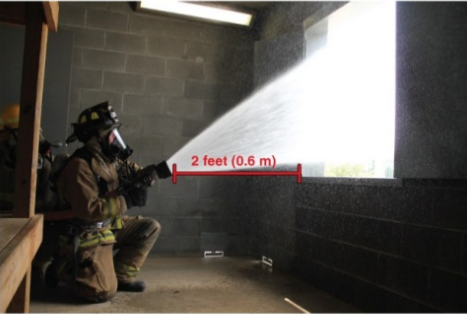
\includegraphics[width=0.5\textwidth]{Figures/Air_Entrainment/Hydraulic_Ventilation.png}
\caption{Hydraulic Ventilation}
\label{fig:Hydraulic_Vent}
\end{figure}
 
Understanding the principals of air entrainment can help firefighters understand how their action will move more or less air. Entrainment based on several different factors including hose stream type, stream length, and nozzle movement, many of which are choices for the firefighter operating the nozzle.

\section{Air Entrainment is Dependent on Hose Stream Type. (Smooth bore, Straight stream, Fog)} 
As a stream breaks up, it creates more droplets, creating more surface area of droplets, which pulls with the droplets more air. As a combination nozzle is adjusted from straight stream, to narrow fog, to wide fog, it entrains more air with the increase in the amount the stream breaks up. If the intent is to move as little air as possible, maintaining a straight stream is desired, however if the nozzle firefighter is interested in moving air, adjusting the nozzle pattern can result in significantly more air movement.

\begin{figure}[!ht]
\centering
\includegraphics[width=0.5\textwidth]{Script_Figures/Entrainment/Opening_Occlusion}
\caption{Straight Stream vs. Narrow Fog}
\label{fig:StraightStream_Fog_Comp}
\end{figure}

When comparing a smooth bore (solid stream) with a combination nozzle straight stream, the amount of dispersion (break up) appreciably the same, resulting in a very similar air entrainment. 

\begin{figure}[!ht]
\centering
\hl{Need Straight Stream \& Smooth Bore Comparison}
\caption{Smooth Bore vs. Straight Stream}
\label{fig:SB_vs_StraightStream}
\end{figure}

\section{Stream Length}
Without the aid of modern personal protective equipment, early fire service nozzles needed to be designed for reach; to provide protection for firefighters by keeping distance between them and the fire. A long reach also meant a greater ability to suppress fires on upper floors without having to drag hoselines through the building. However the further the stream travels the more air will be entrained. 

\begin{figure}[!ht]
\centering
\includegraphics[width=0.5\textwidth]{Script_Figures/Entrainment/Setback_Distance_Comparison.pdf}
\caption{Effect of Stream Length on Entrainment}
\label{fig:Setback}
\end{figure}

Keeping all other factors the same, as a narrow fog is moved back from and opening it exhausts more and more air from the structure. Figure \ref{fig:Setback} shows the different values recorded at 3~ft increments back from a double door. 


If the intent of the nozzle crew is to provide additional air entrainment and in this case exhaust the nozzle should be located as far back in the room as possible. The opposite may be true for a transitional or exterior attack where the intent is to limit the amount of air entrained in the stream as it enters an opening. Having the nozzle positioned as close to the opening as with a straight stream or smooth bore produced little to no entrainment as seen in \ref{fig:Opening_Occlusion}.

\begin{figure}[!ht]
\centering
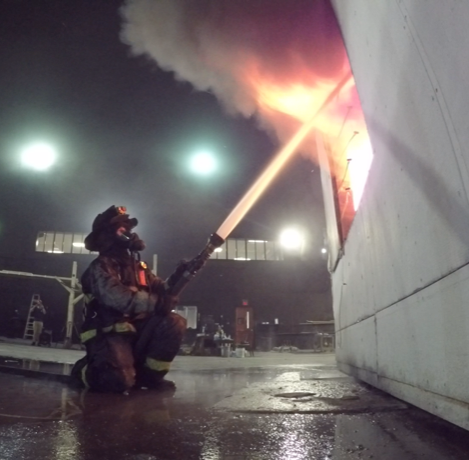
\includegraphics[width=0.4\textwidth]{Figures/Air_Entrainment/Exterior_Attack.png}
\caption{Distance From the Opening has an Impact on Air Entrainment}
\label{fig:ExteriorDist}
\end{figure}


\section{Nozzle Movement}
Nozzle movement or the pattern the firefighter makes with the nozzle does have an impact on the amount of air the hose stream will move. When examining the impact of a fixed nozzle as compared to a moving nozzle, the moving nozzle entrains and therefore moves more air..  Figure \ref{fig:1_5_Interior_Combination_Results_Nozzle_Movements} below shows that a narrow fog `O' pattern yields higher entrainment than a fixed narrow fog pattern and a straight stream `O' pattern yields higher entrainment than a fixed straight stream pattern. 

\begin{figure}[!ht]
	\centering
	\includegraphics[width=4in]{Script_Figures/Entrainment/Total_Entrainment_1_5_Combination_Nozzle_Interior}
	\caption{Figure showing entrainment results of interior 1.5" combination nozzles.}
	\label{fig:1_5_Interior_Combination_Results_Nozzle_Movements}
\end{figure}

The speed at which the nozzle is moved or in this case rotated also has an impact on the amount of air entrained. When the number of revolutions increases from 50/min to 100/min and finally 150/min the amount of air moved increases respectively as shown in Figure \ref{fig:Nozzle_Move_1}.

\begin{figure}[!ht]
\centering
\includegraphics[width=0.5\textwidth]{Script_Figures/Entrainment/Nozzle_Movement_Comparison_1.pdf}
\caption{Impact of Nozzle Movement Speed}
\label{fig:Nozzle_Move_1}
\end{figure}

The type of pattern did not seem to have any impact on the amount of air entrained. When the nozzle was moved in a `O', `Z', or `n' pattern with keeping other variables constant the amount of air entrained was constant (Figure \ref{fig:Pattern_Compare_1}). As a comparison a purposeful `O' pattern is shown adjacent a `Spray and Pray' type pattern in Figure \ref{fig:Pattern_Compare_2} where the amount of air entrained is the same for both patterns. 

\begin{figure}[!ht]
\centering
\includegraphics[width=0.5\textwidth]{Script_Figures/Entrainment/Total_Entrainment_1_5_Smooth_Bore_Nozzle_Interior_Patterns.pdf}
\caption{Pattern Comparison `O', `Z', `n'}
\label{fig:Pattern_Compare_1}
\end{figure}

\begin{figure}[!ht]
\centering
\includegraphics[width=0.5\textwidth]{Script_Figures/Entrainment/Nozzle_Movement_Comparison_2.pdf}
\caption{Purposeful `0' vs. `Spray and Pray'}
\label{fig:Pattern_Compare_2}
\end{figure}

When the intent is to entrain as much as possible, moving the nozzle as rapidly as possible will achieve moe the most air. Additionally if the intent is to move air, a narrow fog moved in an `O' pattern was capable of entraining just as much air as was seen during the positive pressure attack research conducted by UL FSRI \cite{Zevotek_Kerber:2016}. 

\begin{figure}[!ht]
\centering
\includegraphics[width=0.2\textwidth]{Figures/Air_Entrainment/PPV_Comparison.png}
\caption{Single Story Structure Exhaust - PPV \cite{Zevotek_Kerber:2016}}
\label{fig:PPV}
\end{figure}


\section{What did not affect Entrainment}
The nozzle firefighter has several tactical choices on the fire ground 


\chapter{Future Research Needs}

The air entrainment data presented in this report is a one piece of the fire attack study. The intention of this report is to provide preliminary results and insight into the amount of air entrained by hose streams based on pre-determined variables and parameters. The water distribution data and full-scale fire test data are additional components to the study which are needed to create a wholistic understanding. Upon completion of the entire analysis, conclusions can be drawn and tactical considerations can be developed regarding each experimental series, the relationships between the series, and the project in its entirety.  

\chapter{Summary}

The goal of the experiments was quantify water distributions within a room over a set of parameters typical the the fire service. 


\bibliography{UL_general,FireAttackReport}

\clearpage

\appendix

\hl{NEED TO ADD ALL AIRENTRAINMNET TESTS DISCUSSED WITHIN}
% \section{Air Entrainment Figures}
% \label{app:Air_Entrainment_Figures}

% \subsection{Manufacturer Comparison}

% \begin{figure}[!ht]
% \begin{tabular*}{\textwidth}{lr}
% \includegraphics[width=3.5in]{Script_Figures/Entrainment/Manufacturer_1_5_Combination_Nozzle_95gpm_100psi} &
% \includegraphics[width=3.5in]{Script_Figures/Entrainment/Manufacturer_1_5_Combination_Nozzle_150gpm_50psi} \\
% \includegraphics[width=3.5in]{Script_Figures/Entrainment/Manufacturer_1_5_Combination_Nozzle_150gpm_75psi} &
% \includegraphics[width=3.5in]{Script_Figures/Entrainment/Manufacturer_1_5_Combination_Nozzle_150gpm_100psi} \\
% \end{tabular*}
% \caption{Figures showing manufacturer comparison of interior air entrainment results for 1.5 in combination nozzles.}
% \label{fig:1_5_Interior_Combination_Manufacturer}
% \end{figure}

% \clearpage

% \begin{figure}[!ht]
% \begin{tabular*}{\textwidth}{lr}
% \includegraphics[width=3.5in]{Script_Figures/Entrainment/Manufacturer_1_5_Smooth_Bore_Nozzle_7_8_150gpm_50psi} &
% \includegraphics[width=3.5in]{Script_Figures/Entrainment/Manufacturer_1_5_Smooth_Bore_Nozzle_15_16_180gpm_50psi} \\
% \end{tabular*}
% \centering
% \includegraphics[width=3.5in]{Script_Figures/Entrainment/Manufacturer_1_5_Smooth_Bore_Nozzle_1_210gpm_50psi} 
% \caption{Figures showing manufacturer comparison of interior air entrainment results for 1.5 in smooth bore nozzles.}
% \label{fig:1_5_Interior_Smooth_Bore_Manufacturer}
% \end{figure}

% \clearpage

% \subsection{Total Air Entrainment}

% \begin{figure}[!ht]
% \begin{tabular*}{\textwidth}{lr}
% \includegraphics[width=3.5in]{Script_Figures/Entrainment/Total_Entrainment_1_5_Combination_Nozzle_Interior} &
% \includegraphics[width=3.5in]{Script_Figures/Entrainment/Total_Entrainment_1_5_Smooth_Bore_Nozzle_Interior} \\
% \end{tabular*}
% \caption{Figures showing total interior air entrainment results for 1.5 in. nozzles}
% \label{fig:1_5_Interior_Total_Entrainment}
% \end{figure}

% \begin{figure}[!ht]
% \centering
% \includegraphics[width=3.5in]{Script_Figures/Entrainment/Total_Entrainment_1_5_Smooth_Bore_Nozzle_Exterior}
% \caption{Figure showing total exterior air entrainment results for 1.5 in. smooth bore nozzle}
% \label{fig:1_5_Exterior_Total_Entrainment}
% \end{figure}

% \clearpage

% \begin{figure}[!ht]
% \begin{tabular*}{\textwidth}{lr}
% \includegraphics[width=3.5in]{Script_Figures/Entrainment/Total_Entrainment_2_5_Combination_Nozzle_Interior} &
% \includegraphics[width=3.5in]{Script_Figures/Entrainment/Total_Entrainment_2_5_Smooth_Bore_Nozzle_Interior} \\
% \end{tabular*}
% \caption{Figures showing total interior air entrainment results for 2.5 in. nozzles}
% \label{fig:2_5_Interior_Total_Entrainment}
% \end{figure}

% \begin{figure}[!ht]
% \begin{tabular*}{\textwidth}{lr}
% \includegraphics[width=3.5in]{Script_Figures/Entrainment/Total_Entrainment_2_5_Combination_Nozzle_Exterior} &
% \includegraphics[width=3.5in]{Script_Figures/Entrainment/Total_Entrainment_2_5_Smooth_Bore_Nozzle_Exterior} \\
% \end{tabular*}
% \caption{Figures showing total exterior air entrainment results for 2.5 in. nozzles}
% \label{fig:2_5_Exterior_Total_Entrainment}
% \end{figure}

% \clearpage

% \begin{figure}[!ht]
% \begin{tabular*}{\textwidth}{lr}
% \includegraphics[width=3.5in]{Script_Figures/Entrainment/Total_Entrainment_MS_Combination_Nozzle_Interior} &
% \includegraphics[width=3.5in]{Script_Figures/Entrainment/Total_Entrainment_MS_Smooth_Bore_Nozzle_Interior} \\
% \end{tabular*}
% \caption{Figures showing total interior air entrainment results for master stream nozzles}
% \label{fig:MS_Interior_Total_Entrainment}
% \end{figure}

% \begin{figure}[!ht]
% \centering
% \includegraphics[width=3.5in]{Script_Figures/Entrainment/Total_Entrainment_MS_Combination_Nozzle_Interior_500gpm_100psi}
% \caption{Figure showing total interior air entrainment results for combination master stream nozzle}
% \label{fig:MS_Interior_Total_Entrainment_Combination}
% \end{figure}

% \clearpage

% \begin{table}[!ht]
% \centering
% \begin{tabular}{|l|ccc|}
% \hline
% \textbf{Portable Monitor Nozzle Type} & \multicolumn{1}{c|}{\textbf{Interior SS/SB}} & \multicolumn{1}{c|}{\textbf{Interior Fog}} & \textbf{Exterior SS/SB)} \\ \hline
% Combination Nozzle (500 gpm @ 75 psi) & 11582 CFM & 53919 CFM & 26523 CFM \\
% Smooth Bore Nozzle (1 3/8" tip, 500 gpm @ 80 psi) & 6768 CFM & N/A & 31572 CFM \\ \hline
% \end{tabular}
% \caption{Portable Monitor Entrainment Results}
% \label{Portable_Monitor_Entrainment_Results}
% \end{table}

% \clearpage

% \subsection{Ventilation Configuration}

% \begin{figure}[!ht]
% \centering
% \includegraphics[width=6in]{Script_Figures/Entrainment/Vent_Configuration_1_5_Combination_Nozzle_Interior}
% \caption{Figure showing interior air entrainment results for varying vent configurations with a 1.5 in. combination nozzle}
% \label{fig:1_5_Interior_Combination_Vent_Config}
% \end{figure}

% \clearpage

% \begin{figure}[!ht]
% \centering
% \includegraphics[width=6in]{Script_Figures/Entrainment/Vent_Configuration_1_5_Smooth_Bore_Nozzle_Interior}
% \caption{Figure showing interior air entrainment results for varying vent configurations with a 1.5 in. smooth bore nozzle}
% \label{fig:1_5_Interior_Smooth_Bore_Vent_Config}
% \end{figure}

% \clearpage

% \begin{figure}[!ht]
% \centering
% \includegraphics[width=6in]{Script_Figures/Entrainment/Vent_Configuration_1_5_Combination_Nozzle_Exterior}
% \caption{Figure showing exterior air entrainment results for varying vent configurations with a 1.5 in. combination nozzle}
% \label{fig:1_5_Exterior_Combination_Vent_Config}
% \end{figure}

% \clearpage

% \begin{figure}[!ht]
% \centering
% \includegraphics[width=6in]{Script_Figures/Entrainment/Vent_Configuration_1_5_Smooth_Bore_Nozzle_Exterior}
% \caption{Figure showing exterior air entrainment results for varying vent configurations with a 1.5 in. smooth bore nozzle}
% \label{fig:1_5_Exterior_Smooth_Bore_Vent_Config}
% \end{figure}

% \clearpage

% \begin{figure}[!ht]
% \centering
% \includegraphics[width=6in]{Script_Figures/Entrainment/Vent_Configuration_1_5_Combination_Nozzle_Transitional}
% \caption{Figure showing transitional air entrainment results for varying vent configurations with a 1.5 in. combination nozzle}
% \label{fig:1_5_Transitional_Combination_Vent_Config}
% \end{figure}

% \clearpage

% \begin{figure}[!ht]
% \centering
% \includegraphics[width=6in]{Script_Figures/Entrainment/Vent_Configuration_1_5_Smooth_Bore_Nozzle_Transitional}
% \caption{Figure showing transitional air entrainment results for varying vent configurations with a 1.5 in. smooth bore nozzle}
% \label{fig:1_5_Transitional_Smooth_Bore_Vent_Config}
% \end{figure}

% \clearpage

% \begin{figure}[!ht]
% \centering
% \includegraphics[width=6in]{Script_Figures/Entrainment/Vent_Configuration_2_5_Combination_Nozzle_Exterior}
% \caption{Figure showing exterior air entrainment results for varying vent configurations with a 2.5 in. combination nozzle}
% \label{fig:2_5_Exterior_Combination_Vent_Config}
% \end{figure}

% \clearpage

% \begin{figure}[!ht]
% \centering
% \includegraphics[width=6in]{Script_Figures/Entrainment/Vent_Configuration_2_5_Smooth_Bore_Nozzle_Exterior}
% \caption{Figure showing exterior air entrainment results for varying vent configurations with a 2.5 in. smooth bore nozzle}
% \label{fig:2_5_Exterior_Smooth_Bore_Vent_Config}
% \end{figure}

% \clearpage

% \begin{figure}[!ht]
% \centering
% \includegraphics[width=6in]{Script_Figures/Entrainment/Vent_Configuration_PM_Combination_Nozzle_Exterior}
% \caption{Figure showing exterior air entrainment results for varying vent configurations with a portable monitor combination nozzle}
% \label{fig:PM_Exterior_Combination_Vent_Config}
% \end{figure}

% \clearpage

% \begin{figure}[!ht]
% \centering
% \includegraphics[width=6in]{Script_Figures/Entrainment/Vent_Configuration_PM_Smooth_Bore_Nozzle_Exterior}
% \caption{Figure showing exterior air entrainment results for varying vent configurations with a portable monitor smooth bore nozzle}
% \label{fig:PM_Exterior_Smooth_Bore_Vent_Config}
% \end{figure}

% \clearpage

% \subsection{Room Configuration}

% \begin{figure}[!ht]
% \begin{tabular*}{\textwidth}{lr}
% \includegraphics[width=3.5in]{Script_Figures/Entrainment/Room_Configuration_1_5_Combination_Nozzle_Interior_1} &
% \includegraphics[width=3.5in]{Script_Figures/Entrainment/Room_Configuration_1_5_Combination_Nozzle_Interior_4} \\
% \includegraphics[width=3.5in]{Script_Figures/Entrainment/Room_Configuration_1_5_Combination_Nozzle_Interior_2} &
% \includegraphics[width=3.5in]{Script_Figures/Entrainment/Room_Configuration_1_5_Combination_Nozzle_Interior_3} \\
% \end{tabular*}
% \caption{Figures showing the interior air entrainment results for 1.5 in combination nozzles in the room configuration.}
% \label{fig:1_5_Interior_Combination_Room_Config}
% \end{figure}

% \clearpage

% \begin{figure}[!ht]
% \centering
% \includegraphics[width=6in]{Script_Figures/Entrainment/Room_Configuration_1_5_Combination_Nozzle_Exterior}
% \caption{Figure showing the exterior air entrainment results for 1.5 in. combination nozzles in the room configuration.}
% \label{fig:1_5_Exterior_Combination_Room_Config}
% \end{figure}

% \clearpage
\end{document}